\documentclass[fleqn,11pt,openany]{book}

% These two need to be set before including scirun style package
\title{Seg3D Basic Functionality}
\author{Jess Tate, Brett Burton}

% INCLUDE Seg3D STYLE DOCUMENT
\usepackage{seg3d}
\usepackage{marvosym}
\usepackage[rightcaption]{sidecap}
\usepackage{multirow}


\begin{document}

%% starting from SCIRun Doc wiki
%% http://software.sci.utah.edu/SCIRunDocs/index.php/CIBC:Documentation:SCIRun:Tutorial:BioPSE


% CREATE TITLE PAGE --------------------------------------------------
\maketitle

% CHAPTERS ---------------------------------------------------------------

\chapter{Overview}
\label{sec:overview}

\begin{introduction}
This document is meant as a basic reference and walkthrough of the Seg3D layout and functionality.  Specifically, every tool, filter and feature of the software will be addressed in a brief manner.

Note:  If you are looking for a refresher on the available keyboard and mouse shortcuts, there is a list under the `Help' menu of the Seg3D.  
\end{introduction}

\section{About Seg3D}

\begin{figure}
\scalebox{0.3}{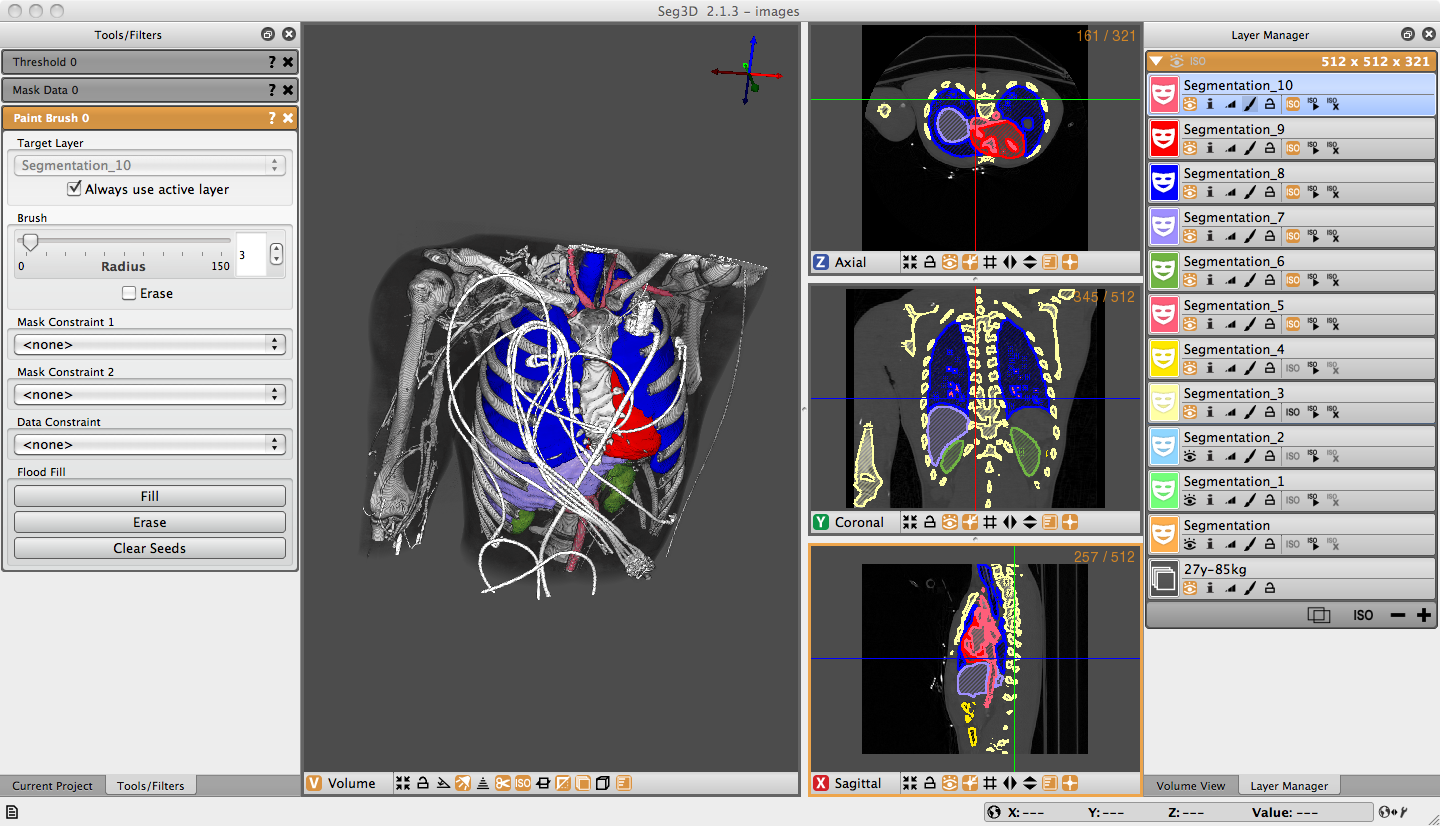
\includegraphics{Seg3DBasicFunctionality_figures/layout.png}}
\caption{Seg3D in use.}\label{fig:layout}
\end{figure}

Seg3D is a lightweight software tool developed for use in visualizing and segmenting image data.  The core intended use of Seg3D involves loading 3D scalar data, such as MRI or CT scans, and generating labels mask to identify various regions of interest in the original image data.  Seg3D facilitates the process using interactive tools such as image processing filters and manual masking techniques.  

In addition to manual segmenting, the current version of Seg3D includes some features that facilitate automated segmenting.  Provenance is a recently added feature which tracks the steps used to create label masks.  This feature allows the user to then repeat the same sets with different parameters using the python and controller windows.  Future extensions of these capabilities will allow for scripting in the terminal and porting to other programs such as SCIRun and Vistrails.

Seg3D is an crucial element of our software suite also involving BioMesh3D and SCIRun that make possible the development of image based computational models.  Label masks generated with Seg3D are used in other software  for such applications as 3D visualization or computational modeling.  BioMesh3D requires a segmentation like those from Seg3D to generate high quality, multi-material computational meshes.  SCIRun is a modular problem solving environment that generates and runs visualization and simulation tasks on segmentations from Seg3D and meshes from BioMesh3D.  This interaction makes Seg3D a key step in image based modeling.

\section{Software requirements}

\subsection{Seg3D \SegthreeDVersion}

Seg3D is distributed as a binary download for Linux, Windows, and OS X. Please visit the SCI software portal ({http://4software.sci.utah.edu} ) to download the latest Seg3D binary. 

%%%%%%%%%%%%%%%%%%%%%%%%%%%%%%%%%%%%%%%%%%%%%%
%%%%%%%%%%%%%%%%%%%%%%%%%%%%%%%%%%%%%%%%%%%%%%%


\chapter{Welcome Screen}
\label{sec:welcome}

\begin{introduction}
Anytime you start Seg3D, users are first presented with the Seg3D welcome screen.  As seen in Figure~\ref{fig:welcome}, the welcome screen consists of the Seg3D splash screen and a menu displaying the available options for starting and continuing a segmentation in Seg3D.  The included options are to load a recent project, open existing project, start a new project, quickly open a file for viewing, and to quit Seg3D.  These options are the same as some of the options in the `File' menu which are explained in this chapter as well as Sec.~\ref{sec:file}.
\end{introduction}

\begin{figure}
\scalebox{0.3}{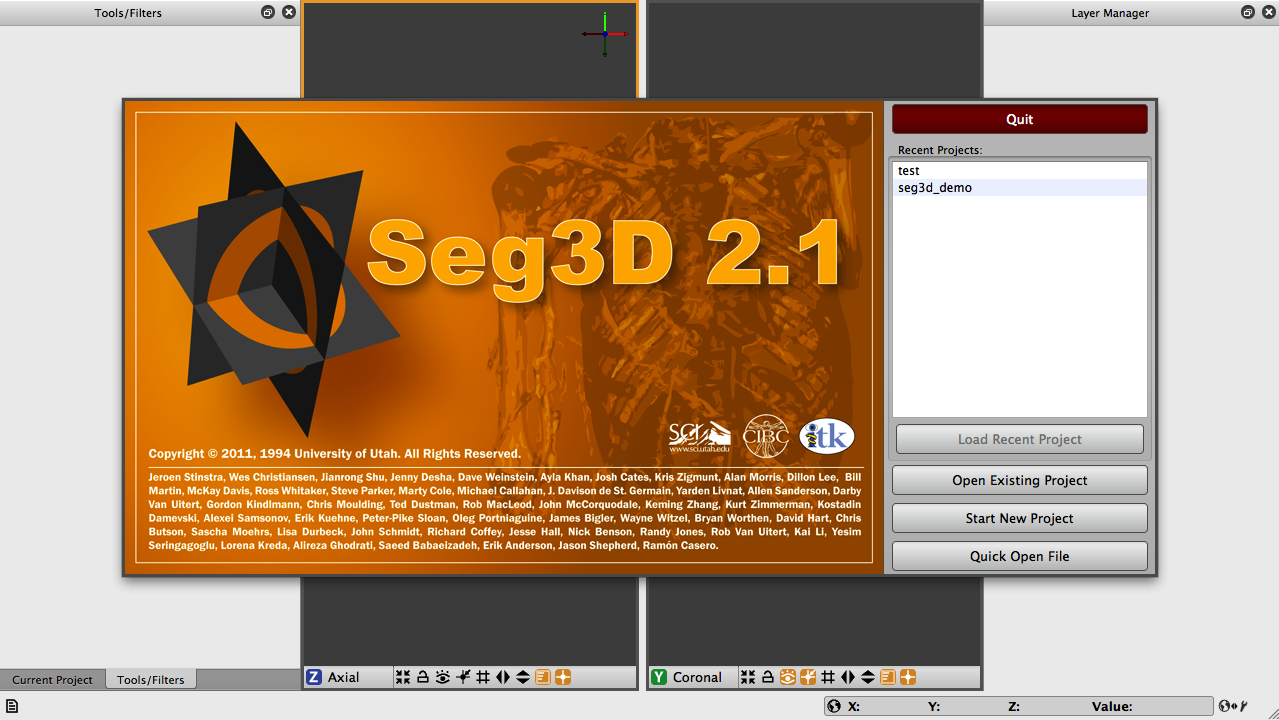
\includegraphics{Seg3DBasicFunctionality_figures/welcome_screen.png}}
\caption{Seg3D welcome screen}\label{fig:welcome}
\end{figure}


\section{Load Recent Project}

This option allows the users to quickly open a project recently opened in Seg3D.  The list of recent projects is shown in the text box above the `Load Recent Project' button (see Figure~\ref{fig:welcome}).  This option will be unavailable unless one of the recent projects in the list is selected.  Updating or reinstalling Seg3D may erase the saved list of recent projects even though the projects still exist.  

\section{Open Existing Project}

This option is the same as `File:Open Project' (sec~\ref{sec:openproject}).  It will open a dialogue window to allow the user to choose an existing *.s3d or *.seg3dproj file to load into Seg3D.  

\section{Start New Project}

This option is the same as `File:New Project' (sec~\ref{sec:newproject}).  It will display the New Project Wizard (Figure~\ref{fig:newproject}), allowing the user to choose a project name and location so that the project can be saved easily and automatically.  

\section{Quick Open File}

This option is the same as `File:Import Layer From Single File...' (sec~\ref{sec:importsinglefile}).  You may choose a file to load into Seg3D for viewing.  All of the filters and tools will be available, but the project can not be saved automatically until a project name is created by using the `File: Save Project As' (sec~\ref{sec:saveprojectas}). 
\\
\\
This option currently does not allow the opening of image stacks.

\section{Quit}

This option will quit Seg3D.  This exist for the rare occasion that you accidentally open Seg3D.  

%%%%%%%%%%%%%%%%%%%%%%%%%%%%%%%%%%%%%%%%%%%%%%%%%%%%%%%%%
%%%%%%%%%%%%%%%%%%%%%%%%%%%%%%%%%%%%%%%%%%%%%%%%%%%%%%%


\chapter{Seg3D Viewer}
\label{sec:viewer}

\begin{introduction}
The Seg3D viewer is the main interface between the users and the software.  This viewer is meant to be highly interactive and intuitive.  Using a combination of mouse functions, keyboard shortcuts, and visual buttons the users can quickly visualize and segment data.  This chapter will describe the functionality of several aspects of the Seg3D viewer including the overall layout of the interface, 2D slice viewer, 3D volume viewer, and the various viewing options available.
\end{introduction}



\begin{figure}[h!]
\scalebox{0.3}{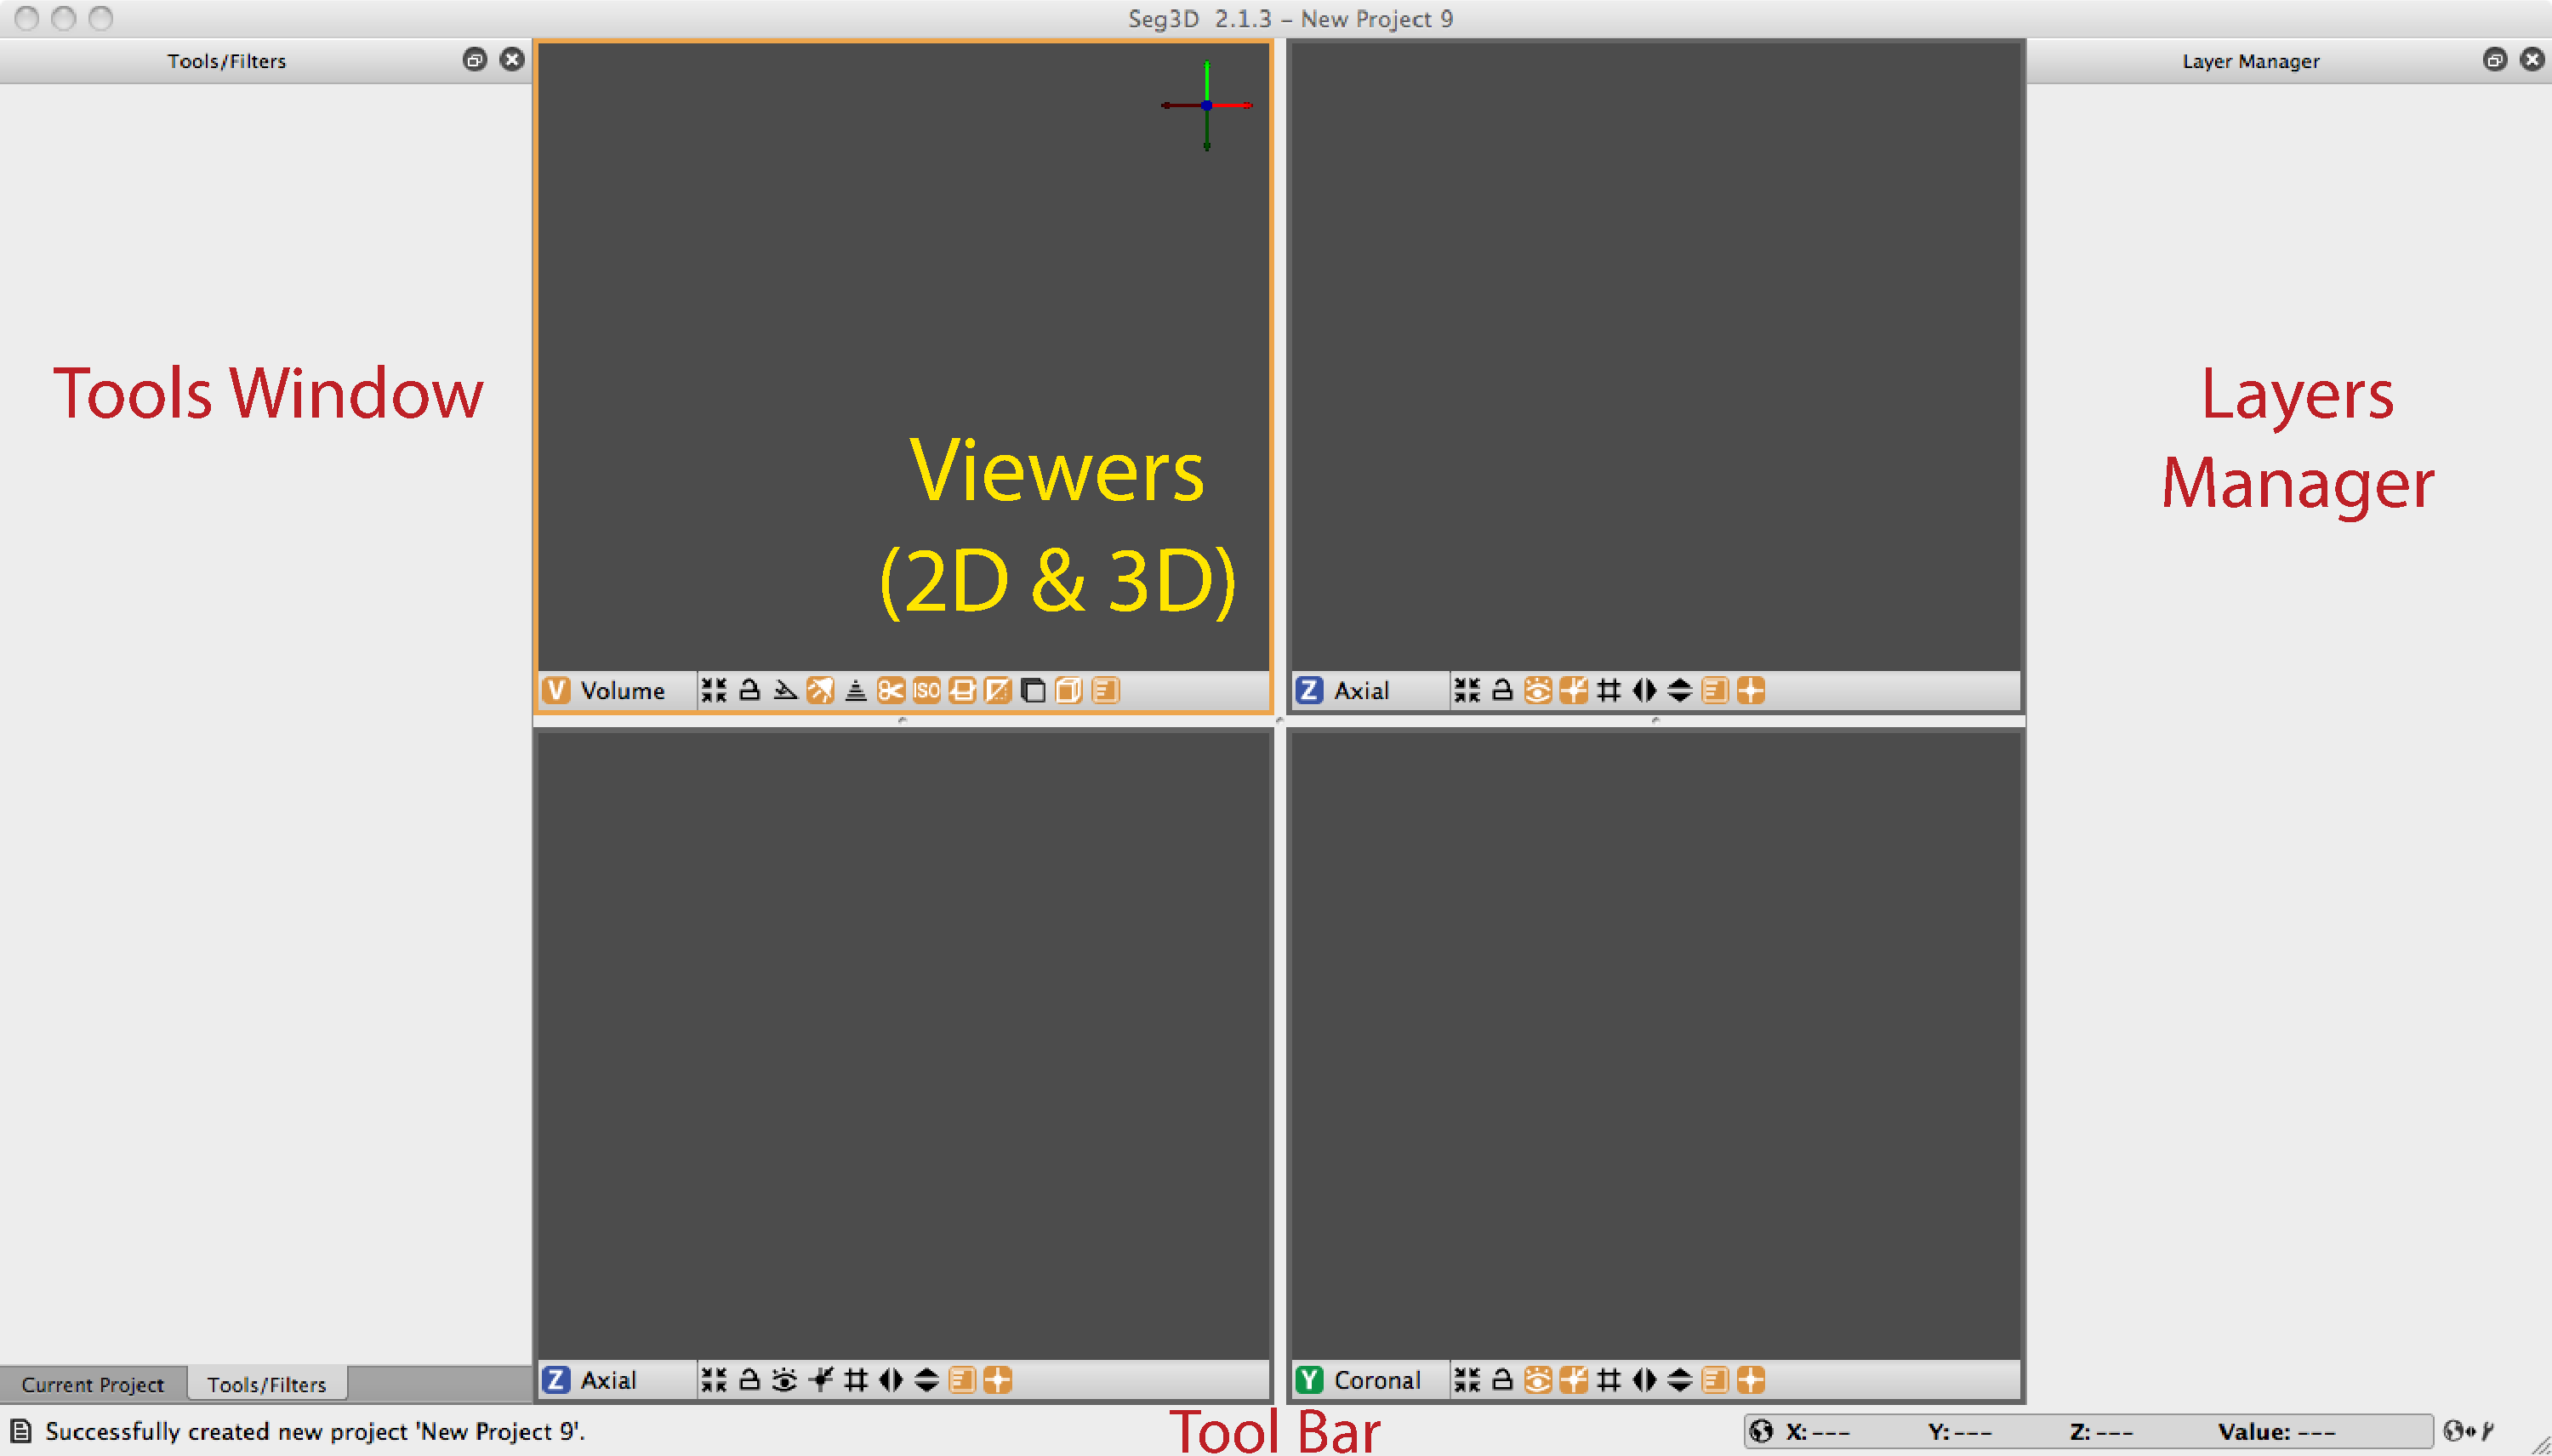
\includegraphics{Seg3DBasicFunctionality_figures/layout_blank.pdf}}
\caption{Seg3D interface}\label{fig:blank}
\end{figure}

The default layout when Seg3D is opened and a new project is created is shown in Figure~\ref{fig:blank}.  As seen from the image the interface for Seg3D consists of a number of viewers (both 2D and 3D), windows to control the functionality of Seg3D, and a tool bar at the bottom of the screen.  

\section{Controlling Windows}
\label{sec:window_control}

The windows on docked the side of the screen can be any of five windows explained in Chapter~\ref{sec:windows} (Project, Tools, Layer Manager, Volume Viewer, and Provenance windows).  Each of these widows can be closed by pressing on the close button \scalebox{0.5}{
\includegraphics{Seg3DBasicFunctionality_figures/close_window.png}} and opened by choosing the window from the `Window' menu or using hot key.  When opened, the window will appear in the last location used, or the default if never opened.  The windows can also be detached from the side (by pressing the detach button \scalebox{0.5}{
\includegraphics{Seg3DBasicFunctionality_figures/dock.png}} and reattached to the side by moving the window close to the side of the Seg3D window, or by double clicking on the window header.  Any detached window can be moved by clicking and dragging on the window header and resized by clicking and dragging on the corner of the window.  Attached windows can also be resized by clicking and dragging on border between it and the viewing panels, but are more limited in the changes allowed.  

\section{Viewer Panels}

As seen in Figure~\ref{fig:blank}, there are a number of viewer panels in Seg3D, though the exact number can be set (see Sec.~\ref{sec:viewing}).  Each of these viewer windows can be changed in size and in type.  The type options are: volume, axial, sagittal, and coronal. The names of the 2D planes can be changed by the user in preferences (Sec.~\ref{sec:preferences}).  You can change the view of each pane by clicking on the view name and choosing the view to change it too.  This is a drop down menu, so you can scroll over the name and the view will also change.  There are also shortcuts to change views (V--Volume, X--Sagittal, Y--Coronal, and Z--Axial) There are several icons in each view panel, as well as mouse and keyboard shortcuts.  The controls for each of the 2D viewers will be described below, as will the controls for the 3D volume viewer.

\subsection{2D Slice Viewer}

Tables~\ref{tab:2dmouse}~\&~\ref{tab:2dkey}  show the mouse and keyboard actions which can be used to control the visualization and manipulation of image and segmentation data.  Though these functions are general, there are tools which used these functions for specify purposes or may otherwise block a couple of these functions, the most prominent example is the scroll wheel in the paint brush tool is used to change brush size.  In this case, you can still scroll through slices by holding shift.  In all cases, an alternative is given in the software.  Also presented in this section is a list and description of the icons presented in the 2D slice viewer (Table~\ref{tab:2dicons}).

\begin{table}[h!]
\label{tab:2dmouse}
\caption{List of mouse functions in the 2D viewers}
\begin{tabular}{|l|l|}
\hline
{\bf Mouse Command} & {\bf Function}\\
\hline
left button drag & Modify brightness and contrast.  \\ &Vertical is contrast, horizontal is brightness. \\
\hline 
scroll up/down & Move up/down a slice\\ &Note: using shift maybe needed while using some tools (like paint brush)\\
\hline
cmd/crtl+right button & Move slices in other planes to intersect at cursor.\\  &Viewers must have the picking icon enabled (Table~\ref{tab:2dicons}).\\
\hline
shift+left button drag & Zan view\\
shift+right button drag & Zoom view in/out\\
\hline
\end{tabular}
\end{table}

\begin{table}[h!]
\label{tab:2dkey}
\caption{List of keyboard actions in the 2D viewers}
\begin{tabular}{|l|l|}
\hline
{\bf Keyboard Action} & {\bf Function}\\
\hline
up arrow,$>$ & move up one slice\\
down arrow,$<$ & move down one slice\\
\hline
shift+up arrow,shift+$>$ & Jump up n slices (set n in preferences)\\
shift+down arrow,shift+$<$ & Jump down n slices (set n in preferences)\\
\hline
left/right arrow & Change active layer to previous/next layer\\
\hline
SPACE & Toggle layer visibility on/off (active layer)\\
\hline
G & Toggle grid visibility\\
\hline
P & Toggle picking state\\
\hline
T & Toggle overlay visibility\\
\hline
L & Toggle lock viewer (to other locked views of the same type)\\
\hline
\end{tabular}
\end{table}

\begin{table}[h!]
\label{tab:2dicons}
\caption{List of icons and actions in the 2D viewers}
\begin{tabular}{|l|l|}
\hline
{\bf Icon} & {\bf Function}\\
\hline
\multirow{2}{*}{ 
\includegraphics[width=0.05\textwidth]{Seg3DBasicFunctionality_figures/AutoViewOff.png} }
& Autoview Icon: This icon forces the panel to fit the objects in viewer with \\
& maximum size.\\
\hline
\multirow{3}{*}{ 
\includegraphics[width=0.05\textwidth]{Seg3DBasicFunctionality_figures/LockOff.png} }
& Lock View Icon: This icon toggles the viewer lock on the panel (shortcut: L). \\ 
& Any changes to any locked viewers will change all the views.  Viewers must \\
& be the same type and each must be locked to use this funtion.\\
\hline
\multirow{2}{*}{ 
\includegraphics[width=0.05\textwidth]{Seg3DBasicFunctionality_figures/VisibleOff.png} }
& Visibility Icon: This icon toggles the visibility of the plane in the 3D volume \\
& viewer.\\
\hline
\multirow{3}{*}{ 
\includegraphics[width=0.05\textwidth]{Seg3DBasicFunctionality_figures/PickingOff.png} }
& Picking Icon: This icon toggles the ability of other planes to pick the slice to \\
& view in the panel.  Only one viewer can have this option enabled.  if only on \\
& of a type of plane, this cannot be disabled.\\
\hline
\multirow{2}{*}{ 
\includegraphics[width=0.05\textwidth]{Seg3DBasicFunctionality_figures/GridOff.png} }
& Grid Icon: This icon toggles the visibility of the grid in the viewer.\\
& \\
\hline
\multirow{2}{*}{ 
\includegraphics[width=0.05\textwidth]{Seg3DBasicFunctionality_figures/FlipHorizOff.png} }
& Flip Horizontal Icon: This icon will horizontally flip the visualization \\
& of the slices in the viewer.\\
\hline
\multirow{2}{*}{ 
\includegraphics[width=0.05\textwidth]{Seg3DBasicFunctionality_figures/FlipVertOff.png} }
& Flip Vertical Icon: This icon will vertically flip the visualization of \\
& the slices in the viewer.\\
\hline
\multirow{2}{*}{ 
\includegraphics[width=0.05\textwidth]{Seg3DBasicFunctionality_figures/OverlayOff.png} }
&  Overlay Icon: This icon will toggle the visibility of the overlay on \\
& the viewer.  This will allow unobstructed viewing of the slices.\\
\hline
\multirow{2}{*}{ 
\includegraphics[width=0.05\textwidth]{Seg3DBasicFunctionality_figures/PickingLinesOff.png} }
& Picking Lines Icon: This icon toggles the visibility of the picking\\
& lines (shows other slices) in the viewing panel.\\
\hline
\end{tabular}
\end{table}

\subsection{3D Volume Viewer}

Though there is no segmentation that can be performed in the 3D volume viewer, it is a very useful function in Seg3D.  It allows the user to see the 3D representation of the original and segmented data.  There are many objects that can be viewed in the 3D viewer such as the 2D slices in 3D, isosurfaces of the segmented data, volume rendering of the image data,  depth cues, and clipping planes.  The purpose of this viewer is to allow you to view your data in as many ways as possible to facilitate segmentation.

\begin{table}[h!]
\label{tab:3dmouse}
\caption{List of mouse functions in the 3D volume viewer}
\begin{tabular}{|l|l|}
\hline
{\bf Mouse Command} & {\bf Function}\\
\hline
left button drag & Pan scene\\
\hline
middle button drag & Rotate scene\\
\hline
right button drag & Zoom in/out on scene\\
\hline
\end{tabular}
\end{table}

\begin{table}[h!]
\label{tab:2dkey}
\caption{List of keyboard actions in the 3D volume viewer}
\begin{tabular}{|l|l|}
\hline
{\bf Keyboard Action} & {\bf Function}\\
\hline
H & Toggle volume lighing\\
\hline
I & Toggle isosurface visibility\\
\hline
T & Toggle overlay visibility\\
\hline
L & Toggle lock viewer (to other locked views of the same type)\\
\hline
\end{tabular}
\end{table}

\begin{table}[h!]
\label{tab:3dicons}
\caption{List of icons and actions in the 3D viewer}
\begin{tabular}{|l|l|}
\hline
{\bf Icon} & {\bf Function}\\
\hline
\multirow{2}{*}{ 
\includegraphics[width=0.05\textwidth]{Seg3DBasicFunctionality_figures/AutoViewOff.png} }
& Autoview Icon: This icon forces the panel to fit the objects in viewer with \\
& maximum size.\\
\hline
\multirow{3}{*}{ 
\includegraphics[width=0.05\textwidth]{Seg3DBasicFunctionality_figures/LockOff.png} }
& Lock View Icon: This icon toggles the viewer lock on the panel (shortcut: L). \\ 
& Any changes to any locked viewers will change all the views.  Viewers must \\
& be the same type and each must be locked to use this funtion.\\
\hline
\multirow{2}{*}{ 
\includegraphics[width=0.05\textwidth]{Seg3DBasicFunctionality_figures/AlignOff.png} }
& Snap to Axis Icon: This icon will move the scene so that the viewing angle is \\
& aligned with the nearest axis.  This will effectively ``straighten'' the scene.\\
\hline
\multirow{3}{*}{ 
\includegraphics[width=0.05\textwidth]{Seg3DBasicFunctionality_figures/LightOff.png} }
& Lighting Icon: This icon toggles the lighting in the 3D viewer.  With the \\
& lighting disable, the images will be shaded as if they were flat, i.e., no \\
& shading.\\
\hline
\multirow{3}{*}{ 
\includegraphics[width=0.05\textwidth]{Seg3DBasicFunctionality_figures/FogOff.png} }
& Depth Cue Icon: This icon toggles the depth cue for the 3d viewer.  This depth\\
& cue acts as fog, blending objects further from the camera into the background.\\
& Fog parameters can be changed in the volume view window (Sec.~\ref{sec:fog}).\\
\hline
\multirow{3}{*}{ 
\includegraphics[width=0.05\textwidth]{Seg3DBasicFunctionality_figures/ClipOff.png} }
& Clipping Icon: This icon toggles the viewing of the clipping planes in the 3D\\
& viewer.  Clipping planes must be created before they can be seen in the volume\\
& viewer (Sec.~\ref{sec:clipping}).\\
\hline
\multirow{3}{*}{ 
\includegraphics[width=0.05\textwidth]{Seg3DBasicFunctionality_figures/IsosurfaceVisibleOff.png} }
& Isosurface Visibility Icon: This icon toggles visibility of the isosurfaces in the\\
& 3D viewer.  This functions effects all the isosurfaces are declared visible in\\
& the layer manager.\\
\hline
\multirow{2}{*}{ 
\includegraphics[width=0.05\textwidth]{Seg3DBasicFunctionality_figures/SlicesVisibleOff.png} }
& Slice Visibility Icon: This icon toggles visibility of the slices in the 3D \\
& viewer.\\
\hline
\multirow{3}{*}{ 
\includegraphics[width=0.05\textwidth]{Seg3DBasicFunctionality_figures/InvisibleSlicesVisibleOff.png} }
& Invisible Slice Visibility Icon: This icon toggles visibility of the invisible\\
& slices in the 3D viewer.  Invisible slices are left when 2D viewers are \\
& destroyed.\\
\hline
\multirow{3}{*}{ 
\includegraphics[width=0.05\textwidth]{Seg3DBasicFunctionality_figures/VolumeRenderingOff.png} }
& Volume Rendering Visibility Icon: This icon toggles visibility of the Volume\\
& Rendering in the 3D viewer.  Volume Rendering must first be created in the\\
& Volume View window (Sec.~\ref{sec:volumerendering})\\
\hline
\multirow{2}{*}{ 
\includegraphics[width=0.05\textwidth]{Seg3DBasicFunctionality_figures/VolumeVisibleOff.png} }
& Volume visibility Icon: This icon toggles visibility of the borders of the active\\ 
& layer in the 3D viewer.\\
\hline
\multirow{2}{*}{ 
\includegraphics[width=0.05\textwidth]{Seg3DBasicFunctionality_figures/OverlayOff.png} }
&  Overlay Icon: This icon will toggle the visibility of the overlay on \\
& the viewer.  This will allow unobstructed viewing of the scene.\\
\hline
\end{tabular}
\end{table}


\clearpage
\section{Tool Bar}

The tool bar located at the bottom of the Seg3D window contains some useful functions.  The first is the message history icon on the left side of the tool bar (Table~\ref{tab:toolbaricons}).   For more information on this window, see Sec.~\ref{sec:messagehistory}.  The other use function is on the right side of the tool bar, the information tool bar.  This tool bar can switch between displaying information about the active layer at the mouse location and a quick menu for the active layers by clicking on the switch tool button (Table~\ref{tab:toolbaricons}).  


\begin{table}[h!]
\label{tab:toolbaricons}
\caption{List of icons and actions in the tool bar at the bottom of Seg3D}
\begin{tabular}{|l|l|}
\hline
{\bf Icon} & {\bf Function}\\
\hline
\multirow{2}{*}{ 
\includegraphics[width=0.05\textwidth]{Seg3DBasicFunctionality_figures/TextOff.png} }
& Message History Icon: Opens Message History window.\\
& \\
\hline
\multirow{3}{*}{ 
\includegraphics[width=0.08\textwidth]{Seg3DBasicFunctionality_figures/SwitchTool.png} }
& Switch Tool Icon:  Switches between displaying location of mouse\\
& in the volume and the quick menu to switch between the active \\
& tools and layers.\\
\hline
\multirow{3}{*}{ 
\includegraphics[width=0.05\textwidth]{Seg3DBasicFunctionality_figures/WorldOff.png} }
& World Icon:  Switches between coordinate system displayed in \\
& the information tool bar.  The options are relative (indexed) and \\
& absolute (world).\\
\hline
\end{tabular}
\end{table}

The information toolbar will show information about the volume at the location indicated by the mouse.  As shown in Figure~\ref{fig:geometricinfo}, the information given is the x, y, and z coordinates and the value of the layer at the mouse position in the selected volume.  By clicking on the world icon (Table~\ref{tab:toolbaricons}), you may toggle between indexed values (relative) and the world values (absolute, considers spacing).  The data shown is changed when the mouse is moved, the active slice is changed, or the active layer is changed.

\begin{figure}[h!]
\scalebox{.7}{
\includegraphics{Seg3DBasicFunctionality_figures/geometric_info.png}}
\caption{Geometric Information shown in the information tool bar.}\label{fig:geometricinfo}
\end{figure}

By clicking on the switch tool icon (Table~\ref{tab:toolbaricons}), the tool bar will display a quick menu for the available tools and layers instead of geometric information.  As seen in Table~\ref{tab:toolbaricons}, this menu will display the active tool and layer.  if the either is clicked, a dropped down menu will appear allowing the user to switch to an open tool or layer.  This can be especially useful in full screen mode.  

\begin{figure}[h!]
\scalebox{.7}{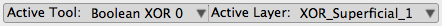
\includegraphics{Seg3DBasicFunctionality_figures/quick_menu.png}}
\caption{Quick menu shown in the information tool bar.}\label{fig:quickmenu}
\end{figure}


\section{Viewing Options}
\label{sec:viewing}

There are several options to change the layout and data viewing in Seg3D.  As mentioned before, several windows can be moved and undocked to customize the layout.  The viewing panels can also be altered so that there are virtually any number (up to sixe) and any size.  Viewing panel sizes can be adjusted by clicking and dragging on the borders.  This may change the sizes of several panels at once, but there are several different configurations available in the `View' menu at the top of the screen.  The various options are explained in the sections following.  

\subsection{Full Screen}

This is a unique and useful viewing option will cause Seg3D to use all of the real estate of whatever screen you are using.  Full screen mode will cover everything else that may be open on your desktop, including the common menus on the top and bottom of the screen.  The top tool bar will reappear if the mouse is held at the top of the screen momentarily, allowing the user to choose any tools or filters desired.  Full screen mode is enable and disabled by clicking on the option in the menu, or by using the shortcut: ctrl/cmd+F.  

\subsection{Only One Viewer}

This and the following viewing options should be self evident.  This option will show only one viewer.  This is useful if you only care about one view at a time because it maximizes screen real estate.  This one viewer can still be switch between the 3 slice orientations and the volume viewer.  

\subsection{One and One}

This will display two viewers side by side.  

\subsection{One and Two}

This will create three viewers,  one bigger one on the left and two smaller ones stacked on the right.  

\subsection{One and Three}

This is the default configuration,  though it can be changed int he preferences.  This generates four viewers, one large one on the left and three smaller ones stacked on the right.  This is a useful configuration because most people do more work in a single view, giving the user one large space to work, but use the other views as references only, so they do not take as much space.

\subsection{Two and Two}

This will generate four viewers of equal size, two on the left and right.  This is useful when you segment in multiple planes simultaneously.

\subsection{Two and Three}

This generates five viewers, two on the left and three on the right.  For when four just doesn't cut it.  

\subsection{Three and Three}

This generates six viewers, the maximum number, three on the left and right.  This is generally used when multiple planes in the same direction are needed.  These planes can be locked together as the user scrolls through them.  

\subsection{Table of Shortcuts}

\begin{table}[h!]
\label{tab:viewerkey}
\caption{Shortcuts for the various viewing options}
\begin{tabular}{|l|l|}
\hline
{\bf Keyboard Action} & {\bf Function}\\
\hline
ctrl/cmd+F & Toggle Full Screen Mode\\
\hline
alt+0 & One viewer only\\
\hline
alt+1 & One and One\\
\hline
alt+2 & One and Two\\
\hline
alt+3 & One and Three\\
\hline
alt+4 & Two and Two\\
\hline
alt+5 & Two and Three\\
\hline
alt+6 & Three and Three\\
\hline
\end{tabular}
\end{table}



%%%%%%%%%%%%%%%%%%%%%%%%%%%%%%%%%%%%%%%%%%%%%%
%---------------------------------------------------------------------------------%%%%%%%%%%%%%%%%%%%%%%%%%%%%%

\chapter{Seg3D Windows}
\label{sec:windows}

\begin{introduction}
In addition to the viewer windows discussed in the above chapter, there are several other
 windows involved in streamlining the user interface of the Seg3D software.  
 Each of these windows can be accessed through the 'Window' drop-down menu.
 By default these windows appear in certain positions defined below, but each can be undocked
 from the Seg3D interface and either left as stand alone windows or repositioned elsewhere on
 the Seg3D application (see Sec.~\ref{sec:window_control}).  
\end{introduction}

\section{Project Window}

\begin{figure}
\scalebox{0.3}{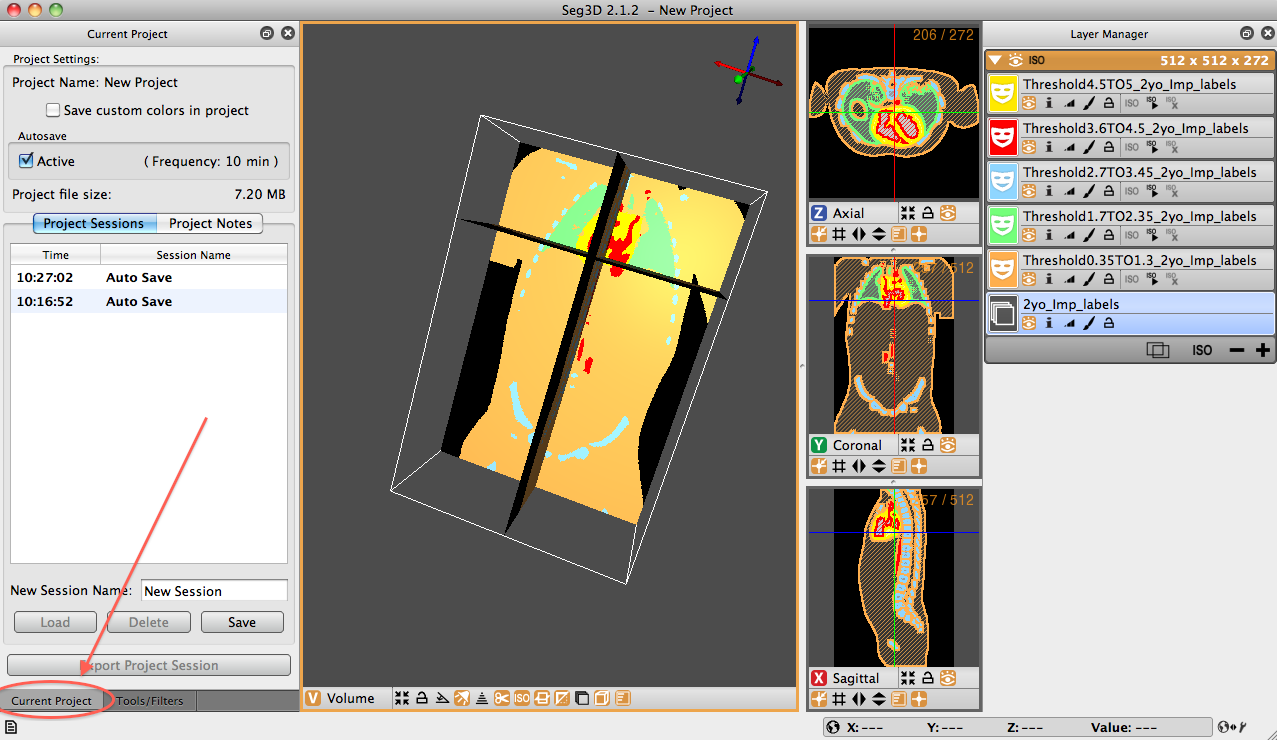
\includegraphics{Seg3DBasicFunctionality_figures/ProjectWindow.png}}
\caption{Project Window}\label{fig:ProjectWindow}
\end{figure}
The project window is one of three windows that is opened by default when Seg3D launches.  
It is located on the left side of the panel and is secondary to the default 'Tools Window' which is also 
located on the left but appears over top of the project window.  
In order to access the window, simply click the tab at the bottom of the left side named 'Current Project' (See Figure \ref{fig:ProjectWindow}) or go to the 'Window' drop down menu, de-select 
'Project Window' and reselect it.

Now you come to the 'Current Project' window.  
The window is divided into two panes.  
At the top of the window is the Project Settings pane.  
The name of the current project is listed.  
Below this is the option to 'Save custom colors in project.'  
This option allows the user to keep the defined colors assigned to specific label masks within the project.  
Below this is an 'Autosave' option. Seg3D autosaves sessions every 10 minutes by default.  
The default time between autosaves can be changed in the general Seg3D preferences.

The second pane holds the 'Project Sessions' and 'Project Notes' panels.  
The project session contains information on the saving of various sessions throughout the work-time in Seg3D - including autosaves.  
These session saves can be selected and loaded at any time.  
Loading a session save does not delete saves that came later.  
To delete, the user must explicitly select the session and push the delete button at the bottom of the pane.  
Additional sessions may also be saved with user specified names.  
The second panel of this pane (the 'Project Notes' panel) allows the user to write notes to along the way.

At any time the user can export the session to a new location - with or without a different name than the original session by clicking the 'Export the Project Session button on the bottom of the  'Current Project' window.

\section{Tools Window}
\begin{figure}[b]
\scalebox{0.3}{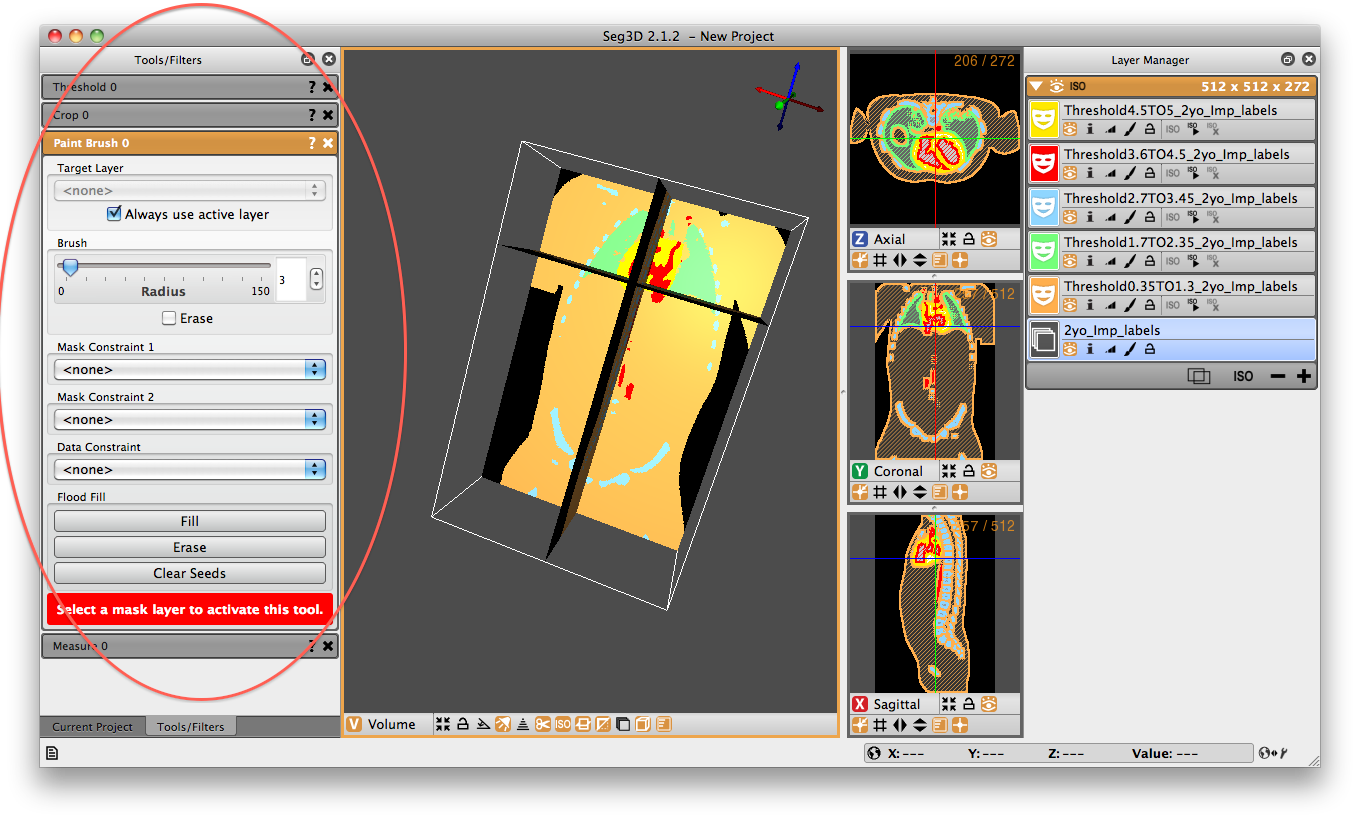
\includegraphics{Seg3DBasicFunctionality_figures/ToolWindow.png}}
\caption{Tools Window}\label{fig:ToolWindow}
\end{figure}
The tools window is another of the three windows that is opened upon Seg3D launch.  
This window is also on the left of the Seg3D panel and is, unlike the project window, is displayed when Seg3D is opened.  
Users can toggle between project and tool windows by selecting the specific tabs at the bottom of the left most window pane.

The tool window houses the current tools that the user has selected from the 'Tools' drop down menu.  
The active tool will be highlighted in orange and will be displayed.  
Inactive tools, that have been opened during the session, will be grayed out and minimized.  
To access one of the other tools, click one of the grayed out items or select it from the 'Tools' drop down menu.  
In Figure \ref{fig:ToolWindow} the 'Paint Brush' tool is active, while the 'Threshold,' 'Crop,' and 'Measure' tools are inactive.



\section{Layer Manager Window}

\begin{figure}[ht!]
\scalebox{0.3}{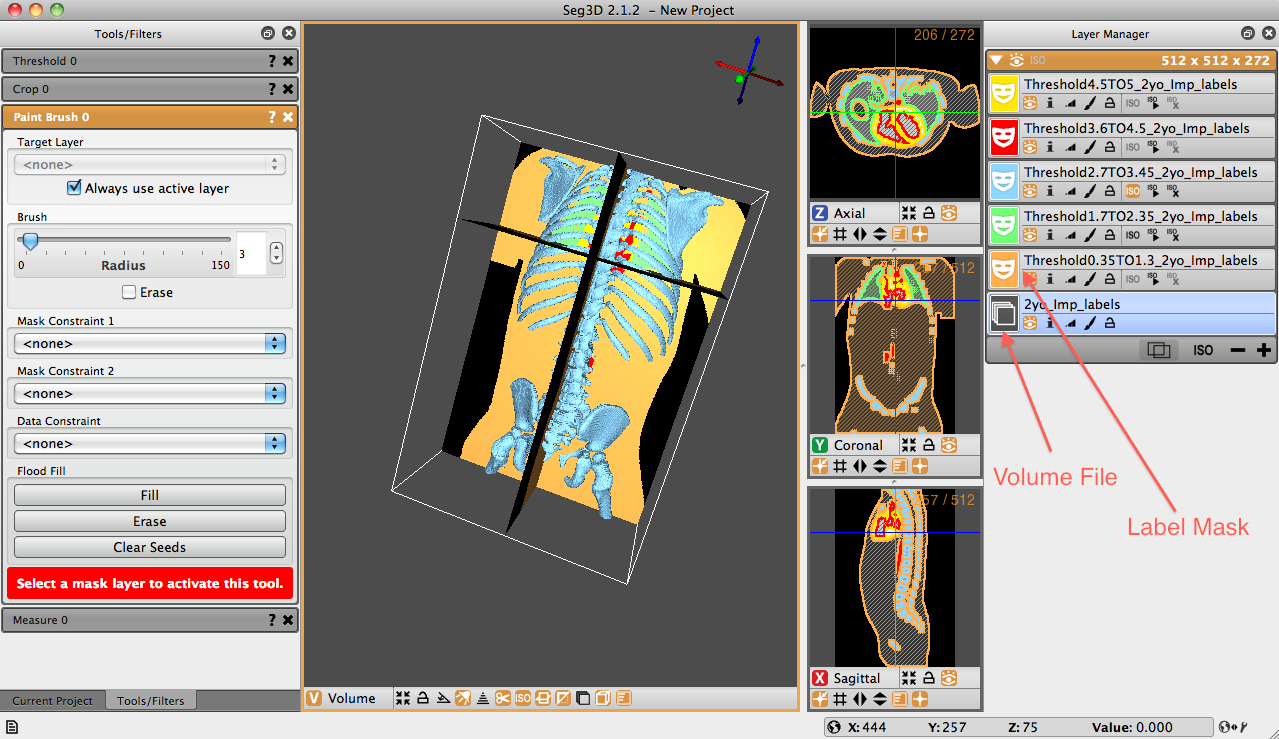
\includegraphics{Seg3DBasicFunctionality_figures/LayerWindow.png}}
\caption{Layer Manager Window}\label{fig:LayerWindow}
\end{figure}

The layer manager window is the last of the three windows that open by default upon launching Seg3D.  
This window is positioned to the right side of the Seg3D window pane and contains all of the mask and volume files involved with the session.  
If a file is not selected when Seg3D launches, this window will be blank, otherwise it will contain the volume and mask surface files associated with the opened file.

A volume file is represented by a gray image with multiple stacked planes.  
A label mask is represented by a colored icon with a white mask in the middle.  
The colors correspond to the label masks seen in the viewer windows.
Names of label masks are, by default, a conglomeration of the tools applied to the original volume.
For example, in the image Figure \ref{fig:LayerWindow} five label masks have been created from the volume file '\verb|2yo_Imp_labels|.' 
The uppermost mask (in yellow) has the name '\verb|Threshold4.5TO5_2yo_Imp_labels|.' 
This name was generated because the threshold tool, with values between 4.5 and 5, was applied to the original volume file. 
If another tool were to be applied on the yellow mask, the new mask would state the name of the tool, followed by the complete name of the yellow label mask.  
Names of masks can be manually changed by clicking the current name and typing in the desired text.

\begin{table}[h!]
\label{tab:layericons}
\caption{List of icons and actions available for each layer.}
\begin{tabular}{|l|l|}
\hline
{\bf Icon} & {\bf Function}\\
\hline
\multirow{3}{*}{ 
\includegraphics[width=0.05\textwidth]{Seg3DBasicFunctionality_figures/VisibleOff.png} }
& Visible Icon: The eye icon displays the current mask.  When the eye is \\
& highlighted the mask is visible in the view plane, when it is not, the mask \\
& is 'turned off.'\\
\hline
\multirow{2}{*}{ \includegraphics[width=0.05\textwidth]{Seg3DBasicFunctionality_figures/infoOff.png} }
& Info Icon: The 'i' icon displays information about the layer.\\
& \\
\hline
\multirow{2}{*}{ 
\includegraphics[width=0.05\textwidth]{Seg3DBasicFunctionality_figures/OpacityOff.png} }
& Opacity Icon: The histogram-looking icon allows the user to change opacity\\
& levels of the layer.\\
\hline
\multirow{2}{*}{ 
\includegraphics[width=0.04\textwidth]{Seg3DBasicFunctionality_figures/AppearanceOff.png} }
& Appearance Icon: The paintbrush-like icon allows the user to change the \\
& layer's appearance.\\
\hline
\multirow{2}{*}{ 
\includegraphics[width=0.05\textwidth]{Seg3DBasicFunctionality_figures/LockOff.png} }
& Lock Icon: The lock icon allows users to lock the layer to further editing.\\
& \\
\hline
\multirow{2}{*}{ 
\includegraphics[width=0.05\textwidth]{Seg3DBasicFunctionality_figures/IsosurfaceVisibleOff.png} }
& Isosurface Visible Icon: This icon toggles visibility of the layers isosurface.  \\
& Isosurfaces must be computed first.\\
\hline
\multirow{3}{*}{ 
\includegraphics[width=0.05\textwidth]{Seg3DBasicFunctionality_figures/IsosurfaceComputeOff.png} }
& Isosurface Compute Icon: This icon generates the isosurface for the mask.\\
& It must be clicked before the IsosurfaceMenu or IsosurfaceDelete icons\\
& become active.\\
\hline
\multirow{2}{*}{ 
\includegraphics[width=0.05\textwidth]{Seg3DBasicFunctionality_figures/IsosurfaceDeleteOff.png} }
& IsosurfaceDelete Icon: This icon deletes active isosurfaces (if the mask\\
& has one).\\
\hline
\end{tabular}
\end{table}

Each volume or mask label has  standard, associated icons below their names.  Table~\ref{tab:layericons} displays and describes each of these icons.  These icons represent tools that are available for each individual layer. 

 \begin{table}[h!]
\label{tab:layertopicons}
\caption{List of icons and actions available at the top of each layer group.}
\begin{tabular}{|l|l|}
\hline
{\bf Icon} & {\bf Function}\\
\hline
\multirow{4}{*}{ 
\includegraphics[width=0.05\textwidth]{Seg3DBasicFunctionality_figures/DownArrow.png} }
& Expanded Layer Group Icon:  This icon indicates that the layer group is \\
& visible, showing all the layers in it.  The layer group can be collapsed, \\
& and expanded again by clicking on this icon. This turns into a right arrow \\
& when collapsed.\\
\hline
\multirow{4}{*}{ 
\includegraphics[width=0.05\textwidth]{Seg3DBasicFunctionality_figures/VisibleOff.png} }
& Visible Icon: This icon will toggle the visibility of all the layers in the group.\\
&  If some of the layers are not visible, this icon will make those layers visible\\
& so that all the layers are visible.  If all layers are visible, this will turn off\\
& visibility.\\
\hline
\multirow{4}{*}{ 
\includegraphics[width=0.05\textwidth]{Seg3DBasicFunctionality_figures/IsosurfaceVisibleOff.png} }
& Isosurface Visibile Icon: This icon toggles visibility of all computed isosurfaces\\
& in the layer group.  If there are computed isosurfaces that are not visible, this \\
& icon will make those visible.  If all computed Isosurfaces are visible, this will \\
& hide them all.\\
\hline
\end{tabular}
\end{table}

 
 Layers in Seg3D are arranged into layer groups.  Layer groups are formed with layers that have the same geometric information, that is the same origin, spacing, and size.  Groups are separated by panels with an orange header.  Generally speaking, most tools and filters requiring more than one input can only operate on layers in the same group (and therefore the same grid geometry).  
 
 \begin{table}[h!]
\label{tab:layerbottomicons}
\caption{List of icons and actions available at the bottom of each layer group.}
\begin{tabular}{|l|l|}
\hline
{\bf Icon} & {\bf Function}\\
\hline
\multirow{4}{*}{ 
\includegraphics[width=0.05\textwidth]{Seg3DBasicFunctionality_figures/DuplicateOff.png} }
& Duplicate Layer Icon:  This icon allows the user to duplicate one or more\\
& layers.  Once this icon is clicked, the user will be prompted to choose the\\
& layers to duplicate by checking the boxes next to the layers.  The duplicated\\
& layers will have the same name with ``copy'' appended to the front.\\ 
\hline
\multirow{4}{*}{ 
\includegraphics[width=0.05\textwidth]{Seg3DBasicFunctionality_figures/IsosurfaceMenuOff.png} }
& Isosurface Menu Icon: This icon will open a menu that allows the user to\\
& change  some of the isosurface rendering parameters for all the isosurfaces\\
& in the layer group.  These parameters are the quality and capping of the \\
& isosurface.\\
\hline
\multirow{4}{*}{ 
\includegraphics[width=0.05\textwidth]{Seg3DBasicFunctionality_figures/Minus.png} }
& Delete Layer Icon: This icon allows the user to delete one or more layer from \\
& the layer group.  When the icon is clicked, the user will be prompted to \\
& choose the layers to delete by clicking the box next to the layer.  There\\
& will be a confirmation window after the selection is made.\\
\hline
\multirow{2}{*}{ 
\includegraphics[width=0.05\textwidth]{Seg3DBasicFunctionality_figures/Add.png} }
& New Layer Icon:  This icon will create a new mask layer that is the same \\
& size as those in the layer group but will be empty.\\
\hline
\end{tabular}
\end{table}

 There are some functions that are operated as a group.  These are indicated by the icons on the top of the pane, in the orange bar (Shown in Tablle~\ref{tab:layertopicons}).  Additionally, there are some other icons at the bottom of the group that control some of the group functions (Table~\ref{tab:layerbottomicons}).  Hovering the cursor over the icon will display the the use of each additional icon.




\section{Volume View Window}
The Volume View Window is not opened by default when Seg3D is opened.  
To open the window, click the 'Window' option in the task bar and select the Volume View option.  
The window may also be toggled by using the key command: Shift+cntrl/cmd+V. 
Once activated, the window will appear on the right and side of the Seg3D panel covering the layer mask window.
To toggle back to the layer mask window, click the Layer Manager tab at the bottom of the page.
The Volume View Window has three separate options for volume displaying.



\subsection{Fog Panel}
\label{sec:fog}


The Fog Panel allows the user to control the fog density.  
In order to observe the effects of fog, the user must activate the Show fog icon on the bottom of the 3D viewer window.
Once active, a fog will be observed on the image.  
The depth of the fog is determined by the distance that the 3-dimensional component is away from the viewer.   
In Figure \ref{fig:FogPanel} the pelvis is tilted away from the viewer.
It is therefore farther from the viewer and has more fog effect applied to it.

Fog density can be tuned by using the slider in the the Volume View Window.  
By default the density value is 1.00.
If the fog density increases, the fogging effect increases.
\begin{figure}[t]
\scalebox{0.3}{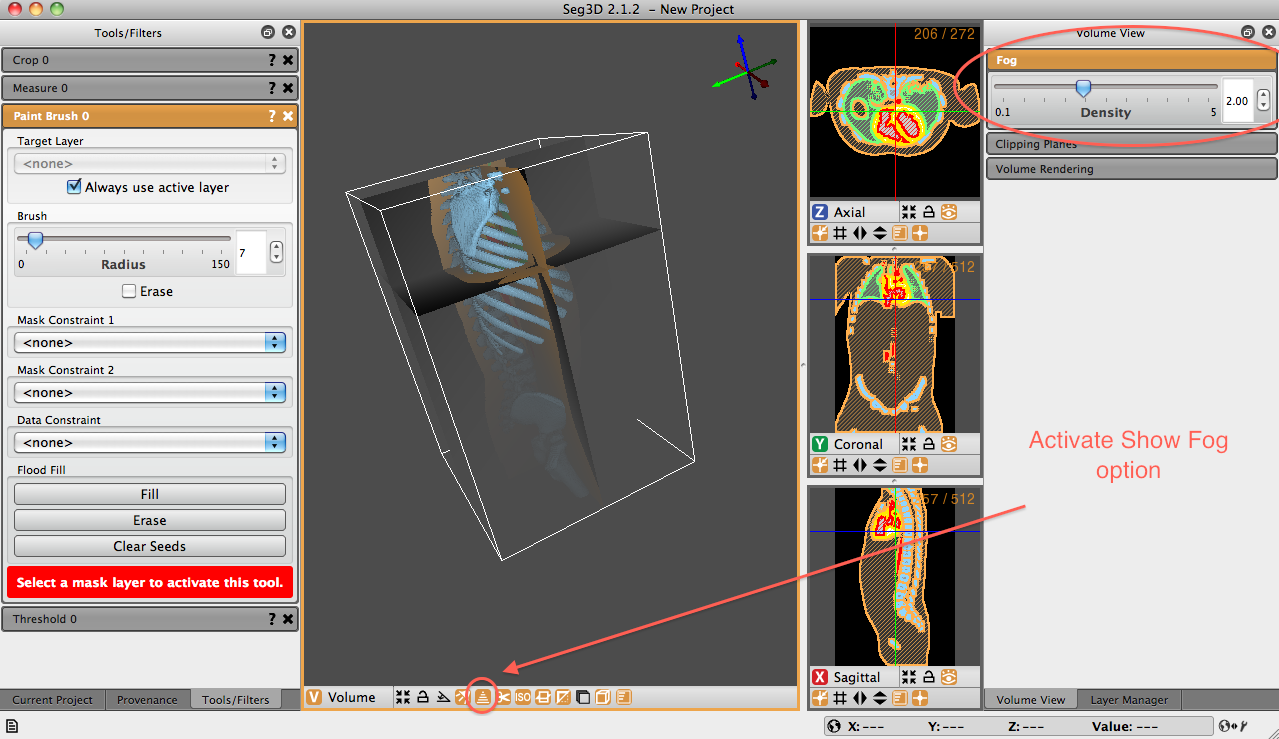
\includegraphics{Seg3DBasicFunctionality_figures/FogPanel.png}}
\caption{Volume View Window - Fog Panel Displayed. The user must activate the Show fog option at the bottom of the viewer window.}\label{fig:FogPanel}
\end{figure}

\subsection{Clipping Planes Panel}
\label{sec:clipping}
The Clipping Planes Panel allows users to define multiple clipping planes with which to clip the volume.  
+ and - signs at the top of the panel represent individual clipping planes.  
The + sign is an enabled clipping plan, while the - sign is disabled.
The clipping panel option in the viewer window is activated by default.

\begin{figure}[b!]
\scalebox{0.3}{\includegraphics{Seg3DBasicFunctionality_figures/ClippingPanel.png}}
\caption{Volume View Window - Clipping Panel Displayed. Show clipping option at the bottom of the viewer window is activated by default.}\label{fig:ClippingPanel}
\end{figure}

Once an clipping plane has been selected, it must be enabled.  Click the 'Enable' checkbox.  
After the plane is enabled, the user is able to define the influence of each cardinal direction on the plane.  
The number 1 in a box indicates that the clipping plane will slice a 45-degree angle within the positive side of that cardinal direction on the 3d viewing window. 
A -1 will clip a -45-degree angle from the negative side.

In order to activate a clip from any cardinal direction, the user must click the slider associated with the desired plane.
If the slider is not clicked, no clipping will take place...even with the clipping plane enabled.
If, say, the z slider is not clicked, no clipping will occur in that plane.
Combining these directional clips allows the user to define a plane that is tipped and tilted in any 3-dimensional direction.
A fourth slider option, the Distance slider, allows the user to define how the position of the clipping plane with respect to the volume.  
If the distance slider is set all the way to the left, no image will be displayed (it will be completely clipped).
If it is set to the right, the entire image will be displayed (no clipping is applied).  
Anything in between will show some clipping of the image.

The final option in the Clipping Planes panel is the option to 'Reverse Normal.'
This option allows the user to reflect the clipping plane.
That is, if the image is clipped within the positive XY plane, the 'Reverse Normal' option will display the clip within the negative XY plane
Figure \ref{fig:ClippingPanel} shows the result of a clipping plane applied in all three cardinal directions.

\subsection{Volume Rendering Panel}
\label{sec:volumerendering}
\begin{figure}[b!]
\scalebox{0.3}{\includegraphics{Seg3DBasicFunctionality_figures/VolRendPanel.png}}
\caption{Volume View Window - Volume Rendering Panel Displayed. Show volume rendering icon at the bottom of the viewer window must be activated.}\label{fig:VolRendPanel}
\end{figure}

The volume rendering panel allows users to generate a volume directly from the volume file, based on the application of transfer functions.
These volume representations are created by extracting values from the transfer functions available and displaying them on a slice-by-slice basis.
If the user zooms the image in closely, each individual slice can be seen (Figure \ref{fig:VolRendOpt}).
The user must define the volume over which they would like to perform the volume rendering.
The user must also make sure that the 'show volume rendering' option is selected at the bottom of the 3D viewer window.

\subsection{Rendering options}

With these two options selected, the user now has three rendering options.
These options are Simple, Faux Shading, and Ambient Occlusion.

\begin{figure}[h!]
\scalebox{0.3}{\includegraphics{Seg3DBasicFunctionality_figures/VolRendOpt.png}}
\caption{Volume Rendering Options - A) Simple B) Faux Shading C) Ambient Occlusion}\label{fig:VolRendOpt}
\end{figure}

\subsubsection{Simple}
The simple rendering strategy gives the user the option to select the Sapling Rate.
The higher the rate, the more accurate the representation of the selected region.
An option in the 'Transfer Function' section of the pane that allows the user to choose 'Solid' transfer function representation changes the appearance by coloring each selected slice to a solid color.
More on this feature will be addressed below.
Note that the images in Figure \ref{fig:VolRendOpt} do not have the solid option selected.

\subsubsection{Faux Shading}
Faux Shading is the same as the simple rendering option with the exception that a simple shading is added to the visible volume.
Where the simple rendering fades regions of the slice to clear (where the 'Solid' transfer function option is NOT selected), the Faux Shading options fade slices to a grayer hue, dependent on where it sits from other 3-dimensionally viewed volumes.
If the 'Solid' feature is selected, the Simple and Faux Shading rendering are the same.

\subsubsection{Ambient Occlusion}
Ambient Occlusion has several additional options.
In addition to the sampling rate, an occlusion angle (range: 0 to 80 degrees) and a sample resolution (range: 1 to 10) are now available.

%Not sure what is these additional options mean.
%The Sample Rate determines the general resolution of the volume.
%The Sample Resolution and the Occlusion angle determine


\subsection{Transfer Function}
Within the transfer function pane, a histogram exists that defines the volumetric image.
The transfer function can be displayed on a Linear or Logarithmic scale.
In the transfer function window, the user can choose to add or delete a feature.
A feature can be dragged into positions defining regions of the histogram that the user wants to render.
The default Feature is a line.  
By clicking and dragging the line, the feature can be moved.
By clicking a point on the line, the individual point can be moved.
Additional points can be added to a feature by clicking anywhere in the histogram panel  that is not already defined by a line, that is, in the gray or black regions.

Each of the features observed can also be enabled/disabled and viewed as solid or graded.
The solid feature (as addressed above) allows the feature to be represented as a graded slice or as a solid one.
Solid slices simply apply the same color saturation to each section of the volume slice.
De-selecting the solid option applies a gradient to the slices, with the outer edge being the brightest color.

Each point and feature can be repositioned, reshaped, and recolored in order to distinguish between defined regions.
To change the color of a feature, select the desired feature and adjust the slider regions below the histogram in the Red/Green/Blue features.
Colors can be used to easily distinguish different features in the volume.
Additionally, each features Ambient and Specular lighting can be adjusted as well as volume shininess is adjustable



\section{Provenance Window}
The Provenance Window is not opened by default when Seg3D is opened. 
To open the window, click the 'Window' option in the task bar and select the Provenance option.  
The window may also be toggled by using the key command: Shift+cntrl/cmd+H.
When the window opens, it will appear on the left side of the Seg3D user interface over top of the 'Current Project' panel and the 'Tools' panel.

The Provenance Window shows the history of the active layer.  
In order to see which actions lead to the current layer, highlight the layer in the 'Layer Window' on the left of the Seg3D display.
Initially, nothing will appear in the Provenance window.
Click the Refresh button at the bottom of the panel and the complete history of that mask will appear.

\begin{figure}[b!]
\scalebox{0.3}{\includegraphics{Seg3DBasicFunctionality_figures/ProvenanceWindow.png}}
\caption{Volume View Window - Clipping Panel Displayed. Show clipping option at the bottom of the viewer window is activated by default.}\label{fig:ProvenanceWindow}
\end{figure}

For example, Figure \ref{fig:ProvenanceWindow} shows an example of a 'FillHoles' Layer.
This layer was was generated by applying a FillHoles tool to the thresholded mask of the lungs.
As can be seen in the Provenance panel, the first step in creating this mask was to Import the volume layer.  
Next, a threshold was taken.  Last, the FillHolesFilter was applied to the Threshold mask.
By selecting one of the steps in the Provenance window, the parameters defining that portion of the mask history will be shown.
For example, by selecting the Threshold option, the thresholding range will be displayed.

\section{Controller Window}
The Controller Window is not opened by default when Seg3D is opened.  To open the window, click the 'Window' option in the task bar and select the Controller option.  The window may also be toggled by using the key command: Shift+cntrl/cmd+C.
Notice the Controller Window option in the window drop-down menu is located below a separator.  
This indicates that the window will open a new pop-up window outside of the general Seg3D user interface.

The Controller window supplies the user with all of the data, variables, history, and logs of the current Seg3D session.
There are four tabs that can be selected in this window:

\subsection{Actions Tab}
The action tab displays all of the actions that have been taken during the Seg3D session.
Console entries can also be made with this feature.
A series of actions area provided in a drop-down menu at the bottom of the window.
Once selected, the action will be placed into a command line to the right of the drop-down menu.
The user can then define the parameters for the action, or simply press enter to see what parameters are required to make the action valid.
If additional parameters are needed to run the action, they will be displayed in the box below the command line.

\subsection{State Variables Tab}
The state variables tab  shows a list of all the state settings for the session.
Settings cannot be edited in this window.

\subsection{Event Log Tab}
The event log shows actions that have been taken on the session since the latest load of the session.
If Seg3D is closed, and then reopened, the event log will only record the history for the newly opened session.
This differs from the action tab in this way, which collects actions for the entire history of the session.
The event log also differs from the action log in that it records all events involved with running Seg3D, not just the actions.
This is also a non-editable tab.

\subsection{Undo/Redo Buffer Tab}
The Undo/Redo Buffer stores past actions for the current open project.
Closing the session will erase the buffers.
In these buffers a user can find the actions, in order, than can be either undone or redone by using Seg3D's Undo and Redo options.


\section{Python Console}
The Python Window is not opened by default when Seg3D is opened.  To open the window, click the 'Window' option in the task bar and select the Python option.  The window may also be toggled by using the key command: Shift+cntrl/cmd+Y.
Notice the Python Window option in the window drop-down menu is located below a separator.  
This indicates that the window will open a new pop-up window outside of the general Seg3D user interface.

The Python Window opens a python scripting console that can be used by advanced users to editing the Seg3D data via python coding.  A treatment of python coding will not be attempted in this document.  For more information on python coding, consult other resources.

\section{Message History Window}
\label{sec:messagehistory}
The Message History Window is not opened by default when Seg3D is opened.  This window is opened by clicking on the message history icon in the bottom left of the screen in the tool bar (Table~\ref{tab:toolbaricons}).    This window will show the messages that Seg3D displays when many functions are performed.  This can be used to track your steps at a high level.  


%%%%%%%%%%%%%%%%%%%%%%%%%%%%%%%%%%%%%%%%%%
%%%%%%%%%%%%%%%%%%%%%%%%%%%%%%%%%%%%%%%%%%%%
%%%%%%%%%%%%%%%%%%%%%%%%%%%%%%%%%%%%%%%%%


\chapter{Basic Program Functions}
\label{sec:functions}

\begin{introduction}
This section gives a brief overview of the options found under the File, Edit, and Help menus. These menus contain options
that allow you to save and open new projects, and set preferences. 

\end{introduction}

\section{File}
\label{sec:file}

\subsection{New Project}
\label{sec:newproject}
The new project option will prompt you to save your current project such that it can be closed. A dialog box will then open
asking for a Project name and a Project Path (Figure~\ref{fig:newproject}).  The Project name will be used to create a folder for all the project data.  The Project path defines the location of this folder, which can be set by typing the path or through a seperate dialogue box by pressing 'Choose Alternate Location'.  The default location for this path can be set in the preferences section discussed below. A new project can also be created using the shortcut cntrl/cmd+N.

\begin{figure}[h!]
\scalebox{0.6}{\includegraphics{Seg3DBasicFunctionality_figures/newProject.png}}
\caption{Project Information window is shown when a new project option is chosen. The project name and location are set in this window}\label{fig:newproject}
\end{figure}

\subsection{Open Project}
\label{sec:openproject}
The open project selection will prompt you to save you current project and open a new project based by selecting it from a file menu.  This function can be called using the shortcut cntrl/cmd+O.

\subsection{Show Project Folder}
This option will open a file menu showing the projects contained in your default project location.  This function can be called using the shortcut shift+cntrl/cmd+O.  The default project location can be changed in Seg3D preferences.

\subsection{Save Project}
If the project as already been given a name and location, this will save the project.  If the project has not yet been named, it will prompt the user for a project name and location.  This function can be called using the shortcut cntrl/cmd+S.

\subsection{Save Project As}
\label{sec:saveprojectas}
This will create a copy of the current project under a new name and project location.  This function can be called using the shortcut shift+cntrl/cmd+S.

\subsection{Launch Another Copy of Seg3D}
This opens a new session of Seg3D.  It does not close the current session, but simply opens another copy.

\subsection{Import Layer From Single File}
\label{sec:importsinglefile}
Data and label maps can be stored in a variety of file formats.  Use this option when the data or label map is stored in one single file.  This function can be called using the shortcut shift+cntrl/cmd+O.

\subsubsection{Import Widget}
After the user selects the file/files to be read, a menu will appear asking the user to define the type of data being read as seen below (Figure~\ref{fig:ImportWidget}).

\begin{figure}[h!]
\scalebox{0.6}{\includegraphics{Seg3DBasicFunctionality_figures/ImportWidget.png}}
\caption{When importing data or label masks, the user is prompted to define the type of data being read.}\label{fig:ImportWidget}
\end{figure}

There are two types of files that can be read by Seg3D: Image data and label maps.  The first selection indicates that the file you wish to read in contains image data.  The next three selections all apply to label maps.  The second selection assumes that all non-zero values are part of a single label map.  The third selection will define each unique value in the file as part of a separate label map. However, the numerical value assigned to represent that label will be incrementally generated by Seg3D rather than assigned from the input file. The fourth selection is similar to the third in that it creates labels based on unique values in the input file.  However, in this case the value used to represent the label is the same as the value being read from the file.

\subsection{Import Layer From Image Series}
Data and label maps can be stored in a variety of file formats.  Use this option when the data or label map is stored in multiple files. See Import Layer From Single File for more information about the Import Widget. This function can be called using the shortcut shift+cntrl/cmd+I.

\subsection{Export Segmentation}
Label maps can be exported in a variety of file formats.  If a layer containing a label map is selected, then the user may select the Export Segmentation option which opens the segmentation dialogue (Figure~\ref{fig:ExportSeg}).

\begin{figure}[h!]
\scalebox{0.6}{\includegraphics{Seg3DBasicFunctionality_figures/ExportSeg.png}}
\caption{This window appears when the user selects export segmentation.  It allows the user to select the layers they wish to export as label masks and the format they wish to export.}\label{fig:ExportSeg}
\end{figure}

This window allows the user to select the layers to export as label masks and the format they wish to export.  The available formats include: .nrrd, .mat (matlab), .tiff, .bmp, .png, .dcm. This function can be called using the shortcut cntrl/cmd+E.  The segmentation may be saved as a single file or as multiple files.  

After choosing a file name (single file only) and location for the segmentation, you will be shown the Export to Segmentation Summary.  This window shows the layers chosen to save as a segmentation.  In the case of saving as a single file,  there is an additional layer (the background, which is the remainder of the volume)  and an option to choose the value to represent each of the layers (Figure~\ref{fig:ExportSeg_2}).  I should be noted that the segmentation will only represent one value per voxel, so if any of the selected layers overlap the higher value will overwrite the region of overlap.  If saving as multiple files, this window will show the names of the layers only.  

\begin{figure}[h!]
\scalebox{0.6}{\includegraphics{Seg3DBasicFunctionality_figures/ExportSeg_2.png}}
\caption{This window appears when the user selects export segmentation and a file is chosen.  This allows the users to choose the labels to use for each material.  }\label{fig:ExportSeg_2}
\end{figure}

\subsection{Export Active Data Layer}

If image data layer is selected, then the user may choose to Export Active Data Layer. This selection opens a file menu window where the user can select the location they wish to save the data file as well as specify the file format.  The available formats include: .nrrd, .dcm, .tiff, .png, .mrc, and .mat (matlab). This function can be called using the shortcut shift+cntrl/cmd+E.

\subsection{Recent Projects}
This menu shows recently opened projects.  These projects can be opened quickly by clicking on the name of the project.

\section{Edit}

\subsection{Undo}
This function allows the user to undo a changes made to the unsaved project.  Changes made to the project are stored
in a buffer, the size of which can be changed under Seg3D preferences. This function can be called using the shortcut cntrl/cmd+Z.


\subsection{Redo}
Redo an operation on a project that was previously undone. This function can be called using the shortcut shift+cntrl/cmd+Z.


\subsection{Copy Mask Slice}
\label{sec:copy}
Copy a single slice from a mask layer which can then be pasted onto other layers. This function can be called using the shortcut cntrl/cmd+C.


\subsection{Paste Mask Slice}
\label{sec:paste}
Paste a previously copied label from one slice of a mask label to all the slices of another mask label. This function can be called using the shortcut cntrl/cmd+V.


\subsection{Punch Through Volume}
\label{sec:punch}
After creating new label data on a single slice of a mask layer, that label can be copied or "punched" to every other slice by
selecting this option. This function can be called using the shortcut cntrl/cmd+P.


\section{Help}
\subsection{Search}
This feature allows you to search all the menus by typing in a search box.

\subsection{Keyboard Shortcuts}
This function opens a list of all the keyboard and mouse shortcuts available in Seg3D.

\section{Preferences}
\label{sec:preferences}
The preference dialogue box can be opened by selection Seg3D-> preferences.  This dialog box
contains four tabs which we will discuss here.


\subsection{General}
The in Seg3D preferences, the general tab allows you to change many details of the "autosave" options.  The user
may turn on the autosave feature and set a frequency for which the project is save.  The "Don't interrupt me" option 
can be turned on so that the auto save does not happen while another operation is being performed. Along with the
frequency the amount of compression used to save each project can be controlled in this tab.  

The "import/export" options allows you to turn on an off a feature that will export a dicom header with all dicoms that are
exported.

The "project" options allow you to change the default project location, change the buffer size, and change how the project
is saved e.g. change if the input files are embedded into the project.

\begin{figure}[h!]
\scalebox{0.6}{\includegraphics{Seg3DBasicFunctionality_figures/Pref_gen.png}}
\caption{The Seg3d preferences under the general tab.}\label{fig:Pref_gen}
\end{figure}


\subsection{View}
Under this tab the user is able to change many of the default view options such as the window layout (1 big window with 3 smaller windows), background color, and Grid size. In addition there are many options to customize what is seen in the visualization window.  At the bottom of this window the user can change the axis labels such that the X,Y, and Z directions
are not fixed to represent Sagittal, Coronal, and Axial, but the user can define which axis label is assigned to each direction.

\begin{figure}[h!]
\scalebox{0.6}{\includegraphics{Seg3DBasicFunctionality_figures/Pref_view.png}}
\caption{The Seg3d preferences under the view tab.}\label{fig:Pref_view}
\end{figure}

\newpage

\subsection{Layers}
Under this tab the user can change the appearance of the label masks. These options include: layer opacity, available colors, mask fill option (striped or solid), and border thickness.

\begin{figure}[h!]
\scalebox{0.6}{\includegraphics{Seg3DBasicFunctionality_figures/Pref_layers.png}}
\caption{The Seg3d preferences under the layers tab.}\label{fig:Pref_layers}
\end{figure}


\subsection{Sidebars/Tools + Filters}
Under this tab the user can select which menus appear on start up and which tools/filters will appear in the 
sidebars.  This intended for the user to customize their user interface to improve the ease of use.

\begin{figure}[h!]
\scalebox{0.6}{\includegraphics{Seg3DBasicFunctionality_figures/Pref_side.png}}
\caption{The Seg3d preferences under the sidebars/tools + filters tab.}\label{fig:Pref_side}
\end{figure}



%-----------------------------------------------------------------------



\chapter{Tools \& Filters}
\label{sec:tools_filters}

\begin{introduction}
 There are many different tools and filters implemented in Seg3D.  These tools and filters are there to attempt several tasks, from reformatting original data, smoothing and de-noising image data, to automatic and manual segmenting.  Every tool and filter will be describe briefly in an effort to provide the user with a list of methods that may be used to segment the data that they have.  These methods have been separated into four categories, general tools, mask filters, data filters, and advanced filters.
 
Most of the tools and filters have a `replace' option.  The default for most of these functions is to create a new layer, but `replace' will cause the new layer to instead replace the old one.  This is very useful in avoiding the generation of multiple layer that are only intermediate steps.  Also, most tools and filters will by default insert the active layer as the primary input.  You may disable this and choose manually which layer to modify.  

 Many of the tools and filters must use a certain type of data as the input, either mask or image data.  If the wrong type of layer is chosen as the input, the tool/filter interface will display a warning message in a red box near the execution button informing you of this.  The tool will also be disabled until the correct type of layer is chosen.  This second feature applies to empty inputs also.  

 A final note is that when tools have multiple inputs, the inputs must all be from the same layer group (geometric grid), with exception of the registration tool.  This ensures that all the voxels in the multiple inputs have corresponding voxels to every other input volume. 

\end{introduction}

\section{Tools}

The tools in this section are useful functions in formatting and segmenting data, but are not usually considered filters.  The formatting tools can be used on either mask or image data, and can generally be performed on more than one layer at once.  The remaining tools are for segmentation.  

\subsection{Copy/Paste}

This tool uses only mask layers as inputs.  It is used to modify mask layers to repeat a slice of interest.  This tool is similar to the basic features found in Sec.~\ref{sec:copy}--\ref{sec:paste}.  The key difference between the edit functions and this tool is that this tool provides more flexibility with the pasting options, offering pasting anywhere from one slice to the whole volume.  The editing options only offer the extremes of pasting a single slice (Sec.~\ref{sec:paste}) or punching a copied slice through the whole volume (Sec.~\ref{sec:punch}).  This tool is most useful to paste multiple slices, but not necessarily the entire volume.  

The Copy/Paste tool has two functions, copy and paste.  The copy buffer only saves one copied slice at a time.  This means that only one slice can be pasted, though it can be pasted to many slices.  The slice to be copied can be specified in two ways, from the viewer (when `use slice from active viewer' is checked) or using a slider and specifying the direction (make sure `use slice from active viewer' is uncheck).  You should be careful using either option to make sure the correct plane is active/selected.  To copy the slice, press the copy button near the middle of the tool window.  

The paste option is a little more complicated, as the user must specify the slice boundaries for the pasting.  This can be done using the provided sliders or by navigating to the slice and pressing the grab from viewer.  The user will need to ensure that the same plane is chosen for the pasting and the copied slice.  Also, it should be noted that the software will not constrain the maximum to be more than the minimum, or vis versa.  if the maximum is lower than the minimum, the tool will still use the slices described and the slices will be pasted.  Press the paste button when the correct slice range is specified to finish.  

This tool will modify the original layer without an option to create a new layer with the action.  

\subsection{Crop}

The crop tool will crop one or more layer to a specified size.  This tool will clip multiple layers from the same group to the same size  by choosing them in the list of layers near the top of the window.  

The size of the new volume can be specified using the sliders in the tool window, or by adjusting the widget in the 2D viewing windows.   The sliders in the tools window will specify the origin and the size of the cropping region.  The buttons over the slider specify which parameter is displayed. It should be noted that you can display the indexed or geometric coordinates by checking/unchecking the `crop in indexed space' option near the bottom of the window.  

The crop widget is shown as a red box in the 2d viewers.  This can be adjusted in any plane by clicking and dragging on the edge to change the size, or in the middle to change the origin.  The mouse pointer will change to indicate which function will be effected.  Press `Crop' to finish cropping the volumes.

\subsection{Flip/Rotate}

The Flip/Rotate tool will flip or rotate 90 degrees one or more layer around a specified axis.  This tool will flip/rotate multiple layers from the same group to the same size  by choosing them in the list of layers near the top of the window.  After choosing the desire layers to flip/rotate, the action is performed when the button for that action is pressed.  There are three flipping options (flipping each axis) and six rotation option (clockwise and counter-clockwise in each plane).  

\subsection{Invert}

This tool will invert the data in a layer to its minimum and maximum, making a negative of the input data.  If performed on a mask layer, this tool will be a mask of everything in the volume besides the original mask.  If performed on image data, the intensities will be reversed so that the dark areas look light and vis versa.

\subsection{Measure}

The measure tool will calculate the distance between two points chosen in the viewer windows.  The points, line segments, and measurements in the 2D viewers and record the measurements in a table in the tools window.   This tool will calculate and retain several different distance allowing the user to copy the measurements to other software (as a text or into a spreadsheet) using the two copy functions in the tool window (selection or all data).  

The user can choose which measurements are visible, change the color, name, and add comments of each of the measurements by double clicking on the parameter in the table, or by highlighting the measurement in the able and clicking the active measurement tab.  A new measurement automatically becomes active.  Using this tab, the user can also center all the active viewers (with picking form other planes allowed) on the points that are in the measurement.  

Back in the general tab, the active layer can be deleted and the opacity of the visualizations in the viewers can be adjusted.  Both tabs allow switching between pixel (indexed) and actual (geometric) distances.  When this is changed in the active measurement tab, it changes all the measurements.  

\begin{table}[h!]
\label{tab:measurekey}
\caption{List of keyboard and mouse actions in the for the Measure Tool}
\begin{tabular}{|l|l|}
\hline
{\bf Action} & {\bf Function}\\
\hline
ctrl/cmd & snap to axis\\
\hline
middle mouse buttom & snap to slice\\
\hline
\end{tabular}
\end{table}


\subsection{Paint Brush}

The paint brush tool a tool that allows full manual creating and editing of mask layers.  This tool allows the user to specify explicitly which pixels to include in the mask label.  This tool can only manipulate existing mask layers (can be empty).   

The paint brush size can be changed with the scroll wheel or in the tools window using the slider.   The left mouse button paints and the right mouse button erases, but this can be reversed by checking the `Erase' option.  

You can constrain the paint brush with other mask layers (up to two) or with a data layer and threshold limits (this is the same as creating a threshold mask layer and using it as a constraint) to limit the pixels that can be painted. 

There is a flood fill and erase function which will fill an area in the slice that is completely surrounded with the mask layer, or delete a connected region.  If no seed points are used with these functions, the entire slice will be filled or erased.  Seed points are chosen with with alt+left mouse button.  

It should be noted that since this tool uses the scroll function to change the paint brush size, it will not also change the slice in the viewer.  To change the slice use the arrow up/down or shift+scroll.  


\begin{table}[h!]
\label{tab:paintkey}
\caption{List of keyboard and mouse actions in the for the Paint Brush Tool}
\begin{tabular}{|l|l|}
\hline
{\bf Action} & {\bf Function}\\
\hline 
left mouse & paint \\
\hline
right mouse & erase\\
\hline
scroll up/down & increase/decrease brush size\\
\hline
alt+left mouse & add seed point\\
\hline
alt+right mouse & remove seed point\\
\hline 
C & clear seed points\\
\hline
F & Paint flood fill\\
\hline
E & Erase flood fill\\ 
\hline
\end{tabular}
\end{table}

\subsection{Point Set Registration}

The point set registration tool will register one mask layer to another mask layer.  This is currently the only tool or filter that will take inputs from two different layer groups as the main purpose of this tool is to allow the user to map a segmentation from one grid to another with a similar mask layer.  The tool attempts to register the entire mask data to another mask data using the iterative closest points method(rigid registration) and will save and display the transform generated for use on the other layers in the registered layer's group.  Since this is an iterative method, the user can set the number of iterations. 

To run this registration, choose for the first input the mask layer in the destination frame (to register to) and the mask to change (register) as the second input.  The ideas is that these would be in separate layer groups.  Clicking the register button will create a new layer in the group of the first input and the transformation will be saved and displayer (translation and rotation).  There will be a list of other mask layers from the second input's group with which the user can select the layer on which to perform the saved transform.  Upon pressing transform, more layers will be generated in the group of the first input layer.  

\subsection{Polyline}

The polyline tool is a tool that allows manual creating and editing of mask layers.  The polyline tool allows the user to define a region of the layer to modify by adding or erasing the data in the region defined by the polyline.  This tool can only manipulate existing mask layers (can be empty).  

The polyline is created by clicking with the left mouse on the 2D viewer.  The polyline can be modified in any plane, but will only fill/erase in the active plane.   The polyline will try to order the new point in between two existing points to make as smooth a shape as possible.  This means that the user should try to place a few points around the edge of the shape desired to create a coarse shape and then fill in the details as needed.  points can be moved with the left mouse button (pointer will turn into a hand) and deleted with the right mouse button.  The whole polyline can be moved with shift+left mouse on one of the points.  

Once the desired region is designated by the polyline, the user can fill the area or delete the mask data in the area.  This tools then is like the paint brush tool, where the brush can be shape in any way.  The polyline will remain as the slice changes, so that the user can modify the existing polyline instead of creating a new one.  If desired, a new polyline can be created by clearing the polyline and starting fresh.  


\begin{table}[h!]
\label{tab:polylinekey}
\caption{List of keyboard and mouse actions in the for the Polyline Tool}
\begin{tabular}{|l|l|}
\hline
{\bf Action} & {\bf Function}\\
\hline 
left mouse & add or move point \\
\hline
right mouse & erase point\\
\hline
shift+left mouse & move polyline (on one of the points)\\
\hline
F & Paint flood fill\\
\hline
E & Erase flood fill\\ 
\hline
\end{tabular}
\end{table}

\subsection{Resample}

The resample tool will allow the user to resample one or more volumes to change the resolution.  This tool can be performed on both mask and data layers.  

The resampling can be set manually using the sliders, or by trying to match the element number of another layer group.  To manually choose the resampling, there are options to resample with the same ratio in every direction (check `Constrain Aspect' option) or to resample each direction independently (must uncheck `Constrain Aspect' option to enable).  To resample to match another group, you must have another layer group loaded.  You may choose the desired group from the drop down menu and the padding value.  

When resample, there is often interpolation of the data needed, especially with image data.  There are several options for interpolation in the resample tool: box, tent, cubic (Catmull-Rom and B-spline), quartic, and guassian.  You may choose the interpolation method in the drop down menu near the bottom of  the tool window.  

\subsection{Speedline}

The speedline tool is similar to the polyline tool in that you use lines to identify a region to segment, but the speedline tool attempts to alter that path between set points to find edges in the image data.  This tool is very useful, but is one of the most complex tools presented in Seg3D.  However, it is not beyond the reach of even a beginner of the software. 

The primary input of the speedline tool is a mask layer which will be altered.  The second input is a speed image, which is similar to a gradient magnitude image.  This speedline image can be created with this tool by choosing the desired image layer in the `Image Data Layer' drop down menu (second one from the top of the tool window) and pressing the `create speed image' button.  The `smooth' option provides additional smoothing to the image and is not needed if the image data has already been smoothed.  When the 'create speed image' button is pressed, a new image layer will be created and the `speed image' option should automatically update to select this new layer.  Otherwise, the user should select the new speed image.  Now the speedline selection can begin.

The selection of the the speedline is virtually identical to the selection of a polyline.  The user will place points and the software will create a shape with those points.  In the speedline case, a new point will be ordered to create as smooth a shape as possible, and the path of the connection will attempt to follow high intensity regions of the speed image (edges of the original image).  Once the desired shape is created, the user can fill the region, or erase it to the mask layer input.  

it should be noted that if the active slice changes, the points will not change, but the connections will still attempt to follow the edge regions of the images.  This can therefore be used to segment multiple slices quickly if the slices do not dramatically change.  The speedline points can be cleared or reset in the tool window.  The user can also set the iterations and termination value to use in the path selection algorithm.  

\begin{table}[h!]
\label{tab:speedlinekey}
\caption{List of keyboard and mouse actions in the for the Speedline Tool}
\begin{tabular}{|l|l|}
\hline
{\bf Action} & {\bf Function}\\
\hline 
left mouse & add or move point \\
\hline
right mouse & erase point\\
\hline
shift+left mouse & move polyline (on one of the points)\\
\hline
F & Paint flood fill\\
\hline
E & Erase flood fill\\ 
\hline
C & Clear seed points\\
\hline
\end{tabular}
\end{table}


\subsection{Threshold}

The threshold tool generates a mask label from an image data volume and the value range to select.  The mask layer created will be a segmentation of the regions in the image data that have intensities in the range specified.  This is one of the most basic semi-automatic tools used in segmentation as it is fast but can also separate contrasted regions very effectively.  

The threshold range can be set in two ways: the slider provided in the tool window will set the maximum and minimum for thresholding or seed points can be placed throughout the volume and the values at those points will set the range to threshold. A preview of the threshold regions will be displayed in the 2D viewers (can be disabled in the tool window).   The opacity of this preview can be set using the provided slider.   The threshold range will also be shown with the image histogram in the tool window. The threshold range and histogram can also be based on a logarithmic scale (more homogenous) or linear scale.  

Using the threshold tool can provide a very good rough segmentation of the region of interest, but may require some editing.  The paint brush and polyline tools are manual ways to remove excess regions in the mask, but the user should also try other mask filters such as connected component and connected component size (and another threshold) to remove stray regions of selected noise.  

\begin{table}[h!]
\label{tab:thresholdkey}
\caption{List of keyboard and mouse actions in the for the threshold Tool}
\begin{tabular}{|l|l|}
\hline
{\bf Action} & {\bf Function}\\
\hline 
M & toggle visibility of the preview mask\\
\hline
\end{tabular}
\end{table}

\subsection{Transform}

The transform tool can be used to translate and scale one or more layers.  This tool can be used on both mask layers and image data layers.  This tool allows the user to change the origin (translate) and the spacing (scale) of multiple layers in a group.  A key use of this tool is to manually transform one layer to match the origin and spacing of a different group, thus including the layer in that group. 

The origin and spacing can be changed in the fields provided, or editing the box widget in the 2D viewer.  To change the box widget, left mouse click and drag in the middle to move the origin, left mouse click and drag on the edge to change the spacing.  The aspect ration of the spacing can be fixed (`Keep Aspect Ratio' option) or the spacing dimension can change independently.  The transform parameters can also be reset so that the original origin and spacing are displayed.  

A preview of one of the checked layers from the list will be shown in the 2D viewer, as well as the box widget.  Both these can be hidden by unchecking the `show preview' and `show border' options, respectively.  If more than one layer is checked, you may choose which layer to preview with the drop down menu provided.  

\section{Mask Filters}

The filters listed in the `Mask Filters' menu all use mask layers as inputs.  These filters, with one exception (Connected Component Size) also produce a new or replaced mask layer.  These tools are simple, yet effective in manipulating mask layer data and can be used in conjunction with the threshold tool at others to create very accurate and nice looking segmentations.

\subsection{Boolean AND}

The boolean AND filter will input two mask layers and output the intersection of the two masks, i.e., the pixels that are masked by both of the two input masks.  

\subsection{Boolean OR}

The boolean OR filter will input two mask layers and output the union of the two masks, i.e., the pixels that are masked by either of the two input masks. 

\subsection{Boolean REMOVE}

The boolean REMOVE filter will input two mask layers and use the second input to remove the intersecting regions from the first.  The result of this can be thought of as the first region minus the second region.  

\subsection{Boolean XOR}

The boolean XOR filter will input two mask layers and output the unique union regions of the two masks, i.e., the pixels that are masked by exactly one of the two input masks. This filter is the same as removing the result of the boolean AND filter from the result of the boolean OR filter.  

\subsection{Connected Component}

The connected component filter finds connected data regions in a mask layer that are coincident to the defined seed points.  This filter can be used to eliminate mask data that is not connected (separated by a blank pixel) from a desired region and can thus reduce noise in the segmentation.  

The seed points are chosen by left clicking in the 2D viewers or deleted by right clicking on existing seed points.  Multiple connected regions can be selected with these seed points.    Another mask can be used as a seed.  Using a mask layer second input field will  cause the filter to find regions from the first input that are overlapping or next to any data in the second input.  Additional seed points can be used or ignored with the `use seed points' option.  

\subsection{Connected Component Size}

The connected component size filter is similar to the connected component filter, but will return a image data layer labeling each connected region with a data value corresponding to its size (logarithmic or linear scale).  This allows the user to manipulate the connected regions in the volume based on size.  For example, thresholding real data can yield several regions of interest that are correct maskings of the data, but may also capture small regions of noise in other areas of the scan.  These small regions of noise can be eliminated using the connected component filter by using the threshold tool on the result.  

\subsection{Fast Binary Dilate -$>$ Erode}

The fast binary dilate -$>$ erode filter will make a label mask bigger (dilate) or smaller (erode).  This filter is very useful in smoothing a mask layer, as performing a dilation and erosion on a mask volume will fill in some of the details on the surface.  This can be desirable if noise is the detail being filled in.  The opposite (erode then dilate) will also smooth, but it will reduce protruding details in the volume.  Either type smoothing should be done carefully as important details may be smoothed in addition to the noise of the segmentation. The amount of smoothing is directly proportional to radius of each step.  The radii are controlled by the slider in the tool window.  

There are several features of this filter that allow high level manipulation of the dilate and erode functions.  First is the ability to add a constraint to the algorithm.  The constraint will not allow the dilation or the erosion of the original mask to exceed the boundary of the constraint mask.  Another feature is to dilate and erode in a specified plane, which can be specified in the viewer or with the drop down menu (disable the `use slice from active viewer' option)  An example of when this is useful is when there is a much bigger spacing in one direction, therefore the 3D dilation extends much further in space in that direction and can cause unwanted closing. 

It should be noted that the edge of the volume provides complications to this filter.  If the mask layer is touching the edge of the volume and erode is performed, the edge slice will perform a 2D erosion only, so that the mask still connects to the edge.  This can  become a problem when the original mask data is near the edge, but not touching, then dilate -$>$ erode is run so that the dilate causes the mask to touch the edge.  The erosion will then leave the mask touching the edge of the volume.

This filter and smooth binary dilate -$>$ erode are similar in function, but are slightly different in the results.  As the name suggests, fast binary dilate -$>$ erode is the faster filter of the two, but the solution may produce corners in the data instead of smooth surfaces.  The runtime of fast binary dilate -$>$ erode is dramatically less and will the results will be indistinguishable with moderate radii and number of eroding and dilating steps.  


\subsection{Fill Holes}

The fill holes filter can be used to fill unmarked regions which are surrounded by a data in a mask layer.  This is useful when automated segmentation techniques leave false negative noise, or regions that should have been marked but aren't.  This filter will  only fill regions that are completely surrounded with mask data.  Therefore, if the filter appears to not work at filter, check the holes and make sure they are not exposed to the background.  The seed points can be used to if there is a hole that is on the edge, but the hole must not be the majority of the edge, i.e. the background.  In this case the seeds are used to identify the background.  Seed points are not needed otherwise.  


\subsection{Smooth Binary Dilate -$>$ Erode}

The fast binary dilate -$>$ erode filter will make a label mask bigger (dilate) or smaller (erode).  This filter is very useful in smoothing a mask layer, as performing a dilation and erosion on a mask volume will fill in some of the details on the surface.  This can be desirable if noise is the detail being filled in.  The opposite (erode then dilate) will also smooth, but it will reduce protruding details in the volume.  Either type smoothing should be done carefully as important details may be smoothed in addition to the noise of the segmentation. The amount of smoothing is directly proportional to radius of each step.  The radii are controlled by the slider in the tool window.  

Though there appears to be several features similar to the fast binary dilate -$>$ erode filter, these have been disabled due to complexity issues from this filter.

It should be noted that the edge of the volume provides complications to this filter.  If the mask layer is touching the edge of the volume and erode is performed, the edge slice will perform a 2D erosion only, so that the mask still connects to the edge.  This can  become a problem when the original mask data is near the edge, but not touching, then dilate -$>$ erode is run so that the dilate causes the mask to touch the edge.  The erosion will then leave the mask touching the edge of the volume.

This filter and fast binary dilate -$>$ erode are similar in function, but are slightly different in the results.  As the name suggests, smooth binary dilate -$>$ erode will produce a smoother surface after each step due to an additional correction in the algorithm.  This additional step adds to runtime dramatically.  You should use this algorithm if the radii used are large, or if the erosion and dilation are performed multiple times each.  

\section{Data Filters}

The filters listed in the `Data Filters' menu all use data layers as inputs.  Most of these filters also produce a new or replaced data layer as the output.  These most of these tools are manipulating image data, such as smoothing and noise reduction, but two of the filters (Neighborhood Connected and Otsu Threshold) generate segmentations (mask layers) based on the data in the data layer.  

\subsection{Arithmetic}

The arithmetic filter allows the user to run basic arithmetic and boolean operations on both image and mask data on a pixel by pixel basis.  This filter can handle up to four inputs and can be used to perform calculate any expression provided by the user(correct syntax is RESULT = \emph{$<$expression$>$};).  There are also many saved expressions that exists as separate filters or tools, the main difference is the functionality to handle more than two inputs.

Any operation can be performed on either type of data, but it should be noted that if a boolean operator is performed it uses zero and non-zero values as the only two possible cases.  This applies to using data layers and also values that may be the summation of mask layers.  

This filter also enables outputs of both data and mask layers.  The filter will switch the output the match the input if the input is changed, but it can be changed afterward.  If there are multiple values in the mathematical result, but mask layer output is chosen, the filter will perform a threshold to try and capture the relevant data in a mask, usually capturing values over zero in the data. 

\subsection{Gaussian Blur}
\label{sec:gaussianblur}

The gaussian blur filter performs a smoothing on the data layer using a discrete gaussian kernel.  For every pixel (except the edges), this filter performs a weighted averaging of the neighboring pixels where the weights are a 3D gaussian distribution centered at the pixel.  This filter will reduce noise by averaging it out, but will also reduce edges.  

The distance parameter set with the slider bar in the tool window determines the size of the neighborhood so that the bigger the distance, the greater the area of averaging and thus more blurring.  Since the distance parameter is the only exposed parameter, the variance is dependent on the distance.

\subsection{Mask Data}

The mask data filter will use the second input of a mask layer to selectively discard (retain) data in a data layer.  The pixels in the data layer that correspond to marked pixels in the mask layer will be kept, and the remaining pixels will be discarded by setting them to some background value.  The background value can be set to zero, the original max or min value, or the new max or min value.  This can be useful in isolating regions of interest and will eliminate noise from outside the region.  This filter could also cause artificial edges and to occur.

\subsection{Mean}\

The mean filter performs a smoothing on the data layer using a discrete step function kernel.  For every pixel (except the edges), this filter performs an averaging of the neighboring pixels.  This filter will reduce noise by averaging it out, but will also reduce edges.  The neighborhood size is controlled by the distance parameter, the greater the distance, the more smoothing.

\subsection{Median}

The median filter is a non-linear filter that will reduce noise (speckle), but may also preserve or enhance sharp boundaries. For every pixel (except the edges), this filter finds the median value of the neighboring pixels and uses this value to replace the original pixel.  This causes the edges to be preserved, if the neighborhood is appropriately sized, while eliminating subtle variations.  

The neighborhood is controlled by the distance parameter.  Though increasing the distance will also increase the smoothing, it is because the size requirement for regions to not be eliminated.  Clear divisions of large regions will increase in contrast and smaller regions will be smoothed out.  

\subsection{Neighborhood Connected}

The neighborhood connected filter is like a combination of the threshold tool and the connected component filter.  The user places seed points in the volume using the 2D viewers (left mouse to place, right mouse to remove).  Then the filter will create a mask layer marking the pixels that are within the data value range of the seed locations that are also connected to the seed points.  This tools is useful in segmenting long and winding structures as long as there is sufficient contrast between the desired structure and the surrounding medium.  

\subsection{Otsu Threshold}

The Otsu threshold filter attempts to cluster data values in a data layer based upon how similar they are and create mask layers identifying the regions of similar data.  This filter provides a good quick segmentation in many cases.  There is a \href{http://en.wikipedia.org/wiki/Otsu's_method}{Wikipedia atricle} containing a good description of the Otsu threshold algorithm.

Using the Ostu threshold filter is simple.  The only parameter in this implementation is the number of thresholds (1 to 4), or the number of divisions in the volume.  The results of this filter are mutually exclusive (no output will mask the same pixel as another layer) and collectively exhaustive (the whole volume will be mask by one of the output layers) so that there will be one more mask layer generated than thresholds used.  A histogram is presented to aid the user in choosing the threshold number.

\section{Advanced Filters}

The filters listed in the `Advance Filters' menu are of various types and purpose.  Filters in this menu either require advanced computational techniques, have multiple parameters, require larger compute times, or a combination of these.  Some of these filter require multiple input of both mask and data layers and may require careful tuning of the parameters to work with different sources of image data.  However, the user should not be discouraged as most of the filters are actually quite easy to use.  This section should explain these filters with the intent to reduce the guess work as much as possible. 

\subsection{Canny Edge}


The Canny edge filter computes the edges in a data layer using a Canny Edge Detection Filter (Canny, J. F. \emph{A computational approach to edge detection}, IEEE PAMI 8(6), 679-698, November 1986).  This filter will output the pixels that are edges in a mask layer.  

This filter is composed of four steps:
\begin{enumerate}
\item Smooth the input image with Gaussian filter.
\item Calculate the second directional derivatives of the smoothed image.
\item Non-Maximum Suppression: the zero-crossings of 2nd derivative are found, and the sign of third derivative is used to find the correct extrema.
\item The hysteresis thresholding is applied to the gradient magnitude (multiplied with zero-crossings) of the smoothed image to find and link edges.
\end{enumerate}

There are two parameters for this filter, distance and minimum threshold.  The distance parameter is the controls the gaussian blurring in the first step and is the same as in the gaussian blur filter (Sec~\ref{sec:gaussianblur}).  Higher distance will result in fewer edges detected and the edges that are detected will likely be thicker.  This is because these edges are being blurred out.  The minimum threshold parameter controls the hysteresis thresholding in the fourth step.  This parameter will set the level of that will count as an edge or not.  This means that a higher minimum threshold will have fewer edges in the result and the remaining edges while more likely be true edges.  

\subsection{Confidence Connected}

The confidence connected filter is similar to the neighborhood connected filter in that it will find connected pixels in a data volume that are statistically similar to pixels surrounding the user defined seed points and output them as a mask layer.  The seed points set in the 2D viewer (left mouse to place, right mouse to remove). 

The pixels neighboring the provided seeds are used to calculate the initial statistics, the variance and mean, then the connected pixels that fit the threshold region defined by the ``Multiplier'' parameter (number of standard deviations from the mean) are selected.  This process is repeated by recalculating the statistics of the selected region and recomputing the connected region based on these new values.  Therefore, the filter can be repeated many times.  

The two parameters in this filter are Iterations and Multiplier.  The Iterations parameter describe the number of times the statistics and connected region are calculated.  Small increases in the number of iterations may not significantly alter the results.  The Multiplier parameter describes the threshold of the pixel intensities as described in the previous paragraph.  The higher the multiplier the more pixels will be selected by the filter.  A small increase in this parameter can very significantly alter the results of the filter.  

Note:  The default values (Iterations=3 and Multiplier=2) should be the best values for most sources of image data.  

\subsection{Curvature Anisotropic Diffusion}

The curvature anisotropic diffusion performs anisotropic diffusion on a data layer using the modified curvature diffusion equation (MCDE).  Anisotropic diffusion filtering is used to reduce noise (or unwanted detail) in images while preserving specific image features, such as edges and is based on the work of Pietro Perona and Jalhandra Malik, \emph{Scale-space and edge detection using anisotropic diffusion}, IEEE PAMI, vol. 12, pp. 629-639, 1990.  The output of this filter is a smoothed data layer.

The parameters for this filter are Iterations and Sensitivity Range.  The iterations parameter will control how many iterations of the filter will be executed.  The more iterations, the smoother the image.  The sensitivity range parameter controls the `diffusion' of the objects in the image, therefore the higher the sensitivity, the more `diffusion' and thus more smoothing.  

\subsection{Distance Map}

The distance map filter will calculate the distance to the surface of a mask  for every pixel in the volume.  This filter will output a distance map as a data layer with the values considered inside the mask marked as negative.  This filter is useful in many applications, such as providing an indicator function for the surface of the mask.  This distance map can also be used to generated a smoother isosurface than may be possible from the original segmentation.  The user may choose between pixel distance or actual distance.  

\subsection{Gradient Anisotropic Diffusion}

The gradient anisotropic diffusion performs anisotropic diffusion on a data layer and uses an additional edge enhancing step to preserve useful features.  Anisotropic diffusion filtering is used to reduce noise (or unwanted detail) in images while preserving specific image features, such as edges and is based on the work of Pietro Perona and Jalhandra Malik, \emph{Scale-space and edge detection using anisotropic diffusion}, IEEE PAMI, vol. 12, pp. 629-639, 1990.  The output of this filter is a smoothed data layer.

The parameters for this filter are Iterations and Sensitivity Range.  The iterations parameter will control how many iterations of the filter will be executed.  The more iterations, the smoother the image.  The sensitivity range parameter controls the `diffusion' of the objects in the image, therefore the higher the sensitivity, the more `diffusion' and thus more smoothing. 

\subsection{Gradient Magnitude}

The gradient magnitude filter will calculate the gradient magnitude of a data layer and output a new or replaced data layer containing the gradient magnitude.   The gradient magnitude is useful as it can highlight regions with edges in the data image because those regions have high gradients.  

This filter is very simple to use because there is only one input and no parameters to adjust, so choose a data layer and go.

\subsection{Histogram Equalization}

The histogram equalization filter will compute the histogram of the data image layer and attempt to transform the image so that the histogram is as flat as possible.  The result of this transformation is most often an increase in contrast that can be considered a visual enhancement of the image.  

There are three parameters to this filter:  Equalization, Histogram Bins, and Bins to Ignore.  

The Equalization parameter provides the most obvious difference to the image.  This filter will combine the original image and the histogram equalized image in the result and this parameter controls the contribution of each.  When the Equalization is 1, the result will be only the equalized image, and when the Equalization is 0, the original image will be returned.  

The Histogram Bins parameter controls the number of bins used in the original histogram used to calculate the transformation, thus this parameter essentially controls the resolution of the intensity transform.   This means that the lower number of bins, the fewer intensity values used in the final image, which can reduce smooth transitions in the image.  Generally, having a higher bin number is better to maintain a smooth image, but the bin number need not be higher than the number of origin possible l intensity values, which is usually dependent on data type.  If the data type is unsigned 8 bit integers, for example, there are 256 intensity values, so more than 256 bins in the filter will not affect the result.  

The Bins to Ignore parameter controls the number of ignored bins in the intensity transformation. When bins are ignored, the pixels that would have been in the bins are moved to the next.  The result of this is that the resulting value range is altered, which could provide additional contrast in some areas.  

\subsection{Intensity Correction}

The intensity correction filter attempts to make the intensity over the data layer homogenous.  This is very useful when dealing with MR images, as the intensity values and contrast can vary over space due to magnetic field variations.  This filter will attempt to fit a spline to average intensity of the image, then to use that spline to equalize the intensity values over the space.  

There are two parameters in this filter, polynomial order and edge sensitivity.  

The polynomial order parameter controls the kind of spline used to correct the image.  A polynomial order of 1 assumes that any changes in intensity is linear through the image.  A higher polynomial order may be needed if there are more complex patterns of intensity variation, such as seemingly isolated regions of high or low intensities.  

The edge sensitivity parameter controls the correction algorithm that prevents artifacts do to edges in the image.  The higher the sensitivity, the less the algorithm will correct for edge artifacts.  As edge sensitivity approaches 0, the algorithm attempts to leave edges unchanged and may suppress the intensity correction altogether.  

\subsection{Segmentation Level Set}

The segmentation level set filter is an iterative segmentation filter that uses a seed volume to find the regions in a data volume that are similar to the original seed.  From mask layer provided as the seed, the statistics of the seeded region are calculated.  The filter will then expand the segmented region to surrounding pixels that match the statistics of the original seeded area.  The propagation may also retract the segmented area in some cases if the seeded areas do not meet the criteria from the threshold range or edge weight.  The filter will continue to expand (or contract) until the iterations are terminated.  

To run this filter, choose a data layer and a mask layer to use as the seed.  The more complete the seed layer is, the fewer the iterations needed to obtain the desired segmentation.  With the proper layers selected, alter the parameters as desired and press `Run Filter'.  A new layer will appear and will update the results of the filter with each iteration.  The user may wait until the filter performs the set number of iterations, or may terminate the process if the desired volume is achieved by pressing `Finish' in the new layer created in the layer window.  

The parameters in this filter to modify are: Iterations, Threshold Range, Curvature Weight, Propagation Weight, and Edge Weight.

The Iterations setting allows the user to set the number of times the filter propagates before terminating.  Since the process can be stopped early while keeping current progress, this number can be set very high if desired.

The Threshold Range parameter controls the intensity values permitted to by included in the propagation of the segmented region.  This range is related to the standard deviation of the original seed volume.  If this parameter is set too low, so of the seed region will be removed as the segmentation propagates.  If this parameter is set to 0, there will be no output data.  This is the most strict parameter, in that all other parameters are met after the threshold range is established.  

The Curvature Weight parameter will control the propagation edge in terms of curvature.  The higher the Curvature Weight, the smother the boundary will be.  It should be noted that curvature can only be weighted in the range set by both the Threshold Range parameter and the Edge Weight parameter, and therefore may not alter the end result if the regions defined by these other parameters is too narrow.  

The Propagation Weight parameter controls how aggressive each iteration will be in determining surrounding pixels that may fit the criteria of the filter.  The high the Propagation Weight, the further the filter searches on each iteration, and therefore the faster it fills a region that matches the criteria. Having a high propagation may also cause the to jump gaps that may not be desired, so it is prudent to reduce the propagation weight in such cases.  The Propagation Weight should be greater than 0 to avoid reduction of the volume.  

The Edge Weight parameter will control how much effect the edges in the data volume effect the propagation pathway.  The Higher the edge weight, the more the filter avoids filling in edges, though the propagation may cause the expansion to fill around the edge.  It should be noted that the filter is very sensitive to this parameter, so that it should be increased with small increments.  Too high of a edge weight could cause holes to appear in what may seem like homogeneous regions.  

On a final note, when the segmentation level set filter is run with the edge and curvature weight at zero and high enough iterations, the result will likely seem similar to the confidence connected filter, but will require much more compute time to reach it.  This can be useful to try when first using this filter on new data, as it will help tune the threshold range better.  With that in mind, suggested parameters for novices are: high Threshold Range (above 2.5, but 5 might be best), high Propagation Weight (Use max unless doing fine tuning or very coarse data), and low Edge Weight (less than 1 unless very smooth data).  The filter is not as sensitive to the curvature weight and the Iterations can be increased as much as desired.  

\end{document}



